\documentclass[12pt]{article}

\usepackage[english]{babel}
\usepackage[utf8x]{inputenc}
\usepackage{amsmath}
\usepackage{graphicx}
\usepackage[colorinlistoftodos]{todonotes}
\usepackage{listings}
\usepackage{glossaries}
\usepackage{placeins}
\usepackage{fixltx2e}
\usepackage{pdfpages}
\usepackage{lastpage}
\usepackage{enumitem}
\usepackage{xcolor}
\usepackage{scrpage2}
\usepackage{scrtime}
\usepackage{parskip}
\usepackage{gensymb}
\usepackage{hyperref} 

\clearscrheadfoot
\pagestyle{scrheadings}
\usepackage[
top    = 2.5cm,
bottom = 3cm,
left   = 3cm,
right  = 3cm]{geometry}
\setcounter{secnumdepth}{4}
\title{Diploma Thesis}


\author{RoboNav}
\date{\today}


%Includes
\setlength{\parindent}{0cm}

\newcommand{\executeiffilenewer}[3]{%
\ifnum\pdfstrcmp{\pdffilemoddate{#1}}%
{\pdffilemoddate{#2}}>0%
{\immediate\write18{#3}}\fi%
}
\newcommand{\includesvg}[1]{%
\executeiffilenewer{#1.svg}{#1.pdf}%
{inkscape -z -D --file=#1.svg --export-pdf=#1.pdf --export-latex}%
\input{#1.pdf_tex}[width=1.0\textwidth]%
}

%Bibtex
\def\BibTeX{{\rm B\kern-.05em{\sc i\kern-.025em b}\kern-.08em
		T\kern-.1667em\lower.7ex\hbox{E}\kern-.125emX}}

%lslisting
\lstdefinestyle{customjava}{
  	language=Java,
  	frame=tlrb,
  	aboveskip=3mm,
  	belowskip=6mm,
  	showstringspaces=false,
  	columns=flexible,
  	basicstyle={\small\ttfamily},
  	numbers=none,
  	numberstyle=\tiny\color{gray},
  	keywordstyle=\color{purple},
  	commentstyle=\color{orange},
  	stringstyle=\color{blue},
  	breaklines=true,
  	breakatwhitespace=true
  	tabsize=3,
}

\lstset{escapechar=@,style=customjava}

%Cite right
\newcommand{\citeof}[2]{{
		\par \begingroup \leftskip=1cm \noindent \textit 
		''#1'' \cite{#2} \\
		\par \endgroup
	}}
	
% Picture insert (UseCase)
% \insertpicture{mik.png}{Some picture}{\cite{bk_key}}{itm:pic1}{0.5}
\newcommand{\insertpicture}[5]{{
	\begin{figure}[!htb]
		\centering\includegraphics[width=#5\textwidth]{#1}
		\caption[#2 #3]{#2}
		\label{#4}
	\end{figure}
	\FloatBarrier
}}
\makeglossaries
\newglossaryentry{json} {name=JSON, description={Java Script Object Notation}}
\newglossaryentry{GPS} {name=GPS, description={Global Positioning System }}
\newglossaryentry{NDGPS} {name=NDGPS, description={National Differential Global Positioning System }}
\newglossaryentry{WADGPS} {name=WADGPS, description={Wide Area Differential Global Positioning System }}
\newglossaryentry{QR} {name=QR, description={Quick Response (Code) }}
\newglossaryentry{RNCP} {name=RNCP, description={RoboNav Communication Protocol}}
\newglossaryentry{TGM} {name=TGM, description={Technologisches Gewerbe Museum / Institute of technology}}
\newglossaryentry{API} {name=API, description={Application Programming Interface}}
\newglossaryentry{JNI} {name=JNI, description={Java Native Interface}}
\newglossaryentry{WiFi} {name=WiFi, description={Wireless Local Area Network}}
\newglossaryentry{DHCP} {name=DHCP, description={Dynamic Host Configuration Protocol}}
\newglossaryentry{IP} {name=IP, description={Internet Protocol}}
\newglossaryentry{MOV} {name=MOV, description={QuickTime Movie (file extension)}}
\newglossaryentry{MPEG4} {name=MPEG4, description={Moving Picture Experts Group 4 (file extension)}}
\newglossaryentry{MJPEG} {name=MJPEG, description={Motion Joint Photographic Experts Group (file extension)}}
\newglossaryentry{JPEG} {name=JPEG, description={Joint Photographic Experts Group (file extension)}}
\newglossaryentry{CPU} {name=CPU, description={Central Processing Unit}}
\newglossaryentry{GHz} {name=GHz, description={Gigahertz (thousands of MHz)}}
\newglossaryentry{ROS} {name=ROS, description={Robot Operationg System}}
\newglossaryentry{GNUGPL} {name=GNU GPL, description={Gnu's Not Unix General Public License}}
\newglossaryentry{BSD} {name=BSD, description={Berkeley Software Distribution}}
\newglossaryentry{GUI} {name=GUI, description={Graphical User Interface}}
\newglossaryentry{DFT} {name=DFT, description={Discrete Fourier Transform}}
\newglossaryentry{RGB} {name=RGB, description={Red Green Blue}}
\newglossaryentry{UML} {name=UML, description={Unified Modeling Language}}
\newglossaryentry{MRDS} {name=MRDS, description={Microsoft Robotics Developer Studio}}
\newglossaryentry{IDE} {name=IDE, description={Integrated Development Environment}}
\newglossaryentry{FXML} {name=FXML, description={JavaFX - Extensible Markup Language file}}
\newglossaryentry{XML} {name=XML, description={Extensible Markup Language}}
\newglossaryentry{MVC} {name=MVC, description={Model View Control}}
\newglossaryentry{CSS} {name=CSS, description={Cascading Style Sheet}}

\renewcommand*\glspostdescription{\dotfill}




\begin{document}


\begin{titlepage}
\begin{center}

% Additional to first page

\includegraphics[width=0.7\textwidth]{images/logo}\\

\LARGE TGM - HTBLuVA Wien XX \\ IT Abteilung  \\[1.5cm]

% Title
\rule{1.0\textwidth}{1mm}
{ \huge \bfseries \\[0.4cm]  \huge Diplomarbeit \\ \LARGE Urban Green \\[0.4cm] }
\rule{1.0\textwidth}{1mm}

{ \huge Ramin Bahadoorifar \\ Matthias Schwebler \\ Samuel Schober \\ Konrad Kelc \\[0.4cm] }



\noindent 


\vfill

% Bottom of the page
{\small Version: \today ~at  \thistime    }
\end{center}

%\end{center}
\end{titlepage}


%HEADER AND FOOTER
\pagenumbering{Roman}
\ohead{\headmark}
\ifoot{© RoboNav - 2014/15}
\ofoot{\pagemark}

\newpage %----------------------------------------------------------------------------------------------
{\small\color{white}.}
\vspace{-0.7cm}
\tableofcontents

\newpage %----------------------------------------------------------------------------------------------
% Affirmation
%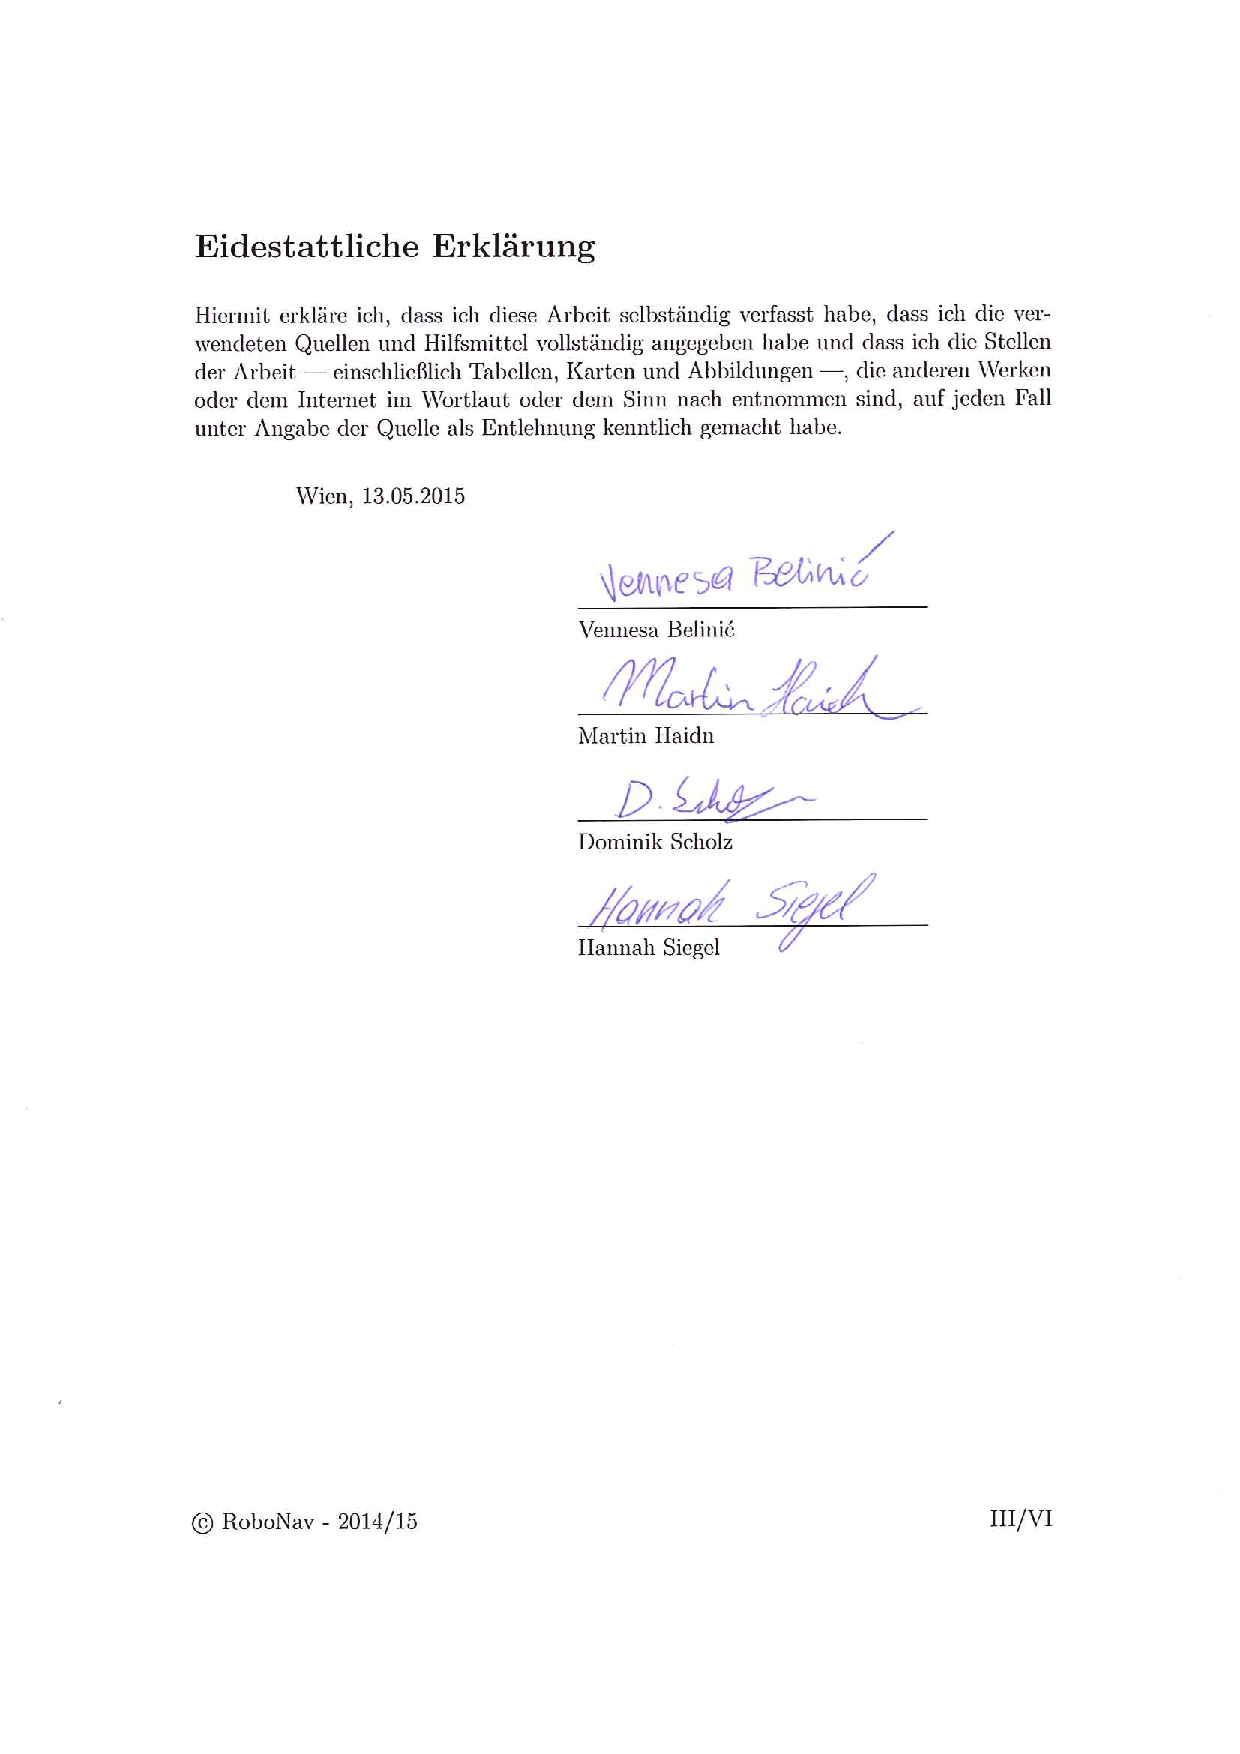
\includepdf[scale=1.2,pages=-]{documents/soor}
%\newpage
\section*{Abstract}
\cfoot{Matthias Schwebler}

*Abstract DE auf enlisch \"ubersetzen*

\newpage
\section*{Kurzfassung}
\cfoot{Matthias Schwebler}

Dieses Diplomprojekt, wird in Kooperation mit der Firma "Ponix Systems" durchgef\"uhrt und handelt \"uber die Entwicklung eines Low-Cost Prototypen eines Aquaponik Systems f\"ur den Heimgebrauch um dem globalen Trend der Umweltverbesserung zu folgen. Das Hauptziel unseres Projektes ist es, die derzeitige Marktl\"ucke von Aquaponik Systemen in Mitteleuropa zu f\"ullen. Daf\"ur wird ein pflegeleichtes \"Okosystem - bestehend aus einem Aquarium und einem Beet - entwickelt und auf die \"Uberwachung und Automatisierung optimiert. Dazu werden diverse Sensoren, Aktoren und Single Board Computer verbaut, welche die Regulierung der Parameter des Systems \"ubernehmen. Die Daten des Aquariums bzw. der Pflanzen werden an einen zentralen Server geleitet und dort persistiert um gegebenenfalls gew\"unschte Diagramme und Graphen zu erstellen. F\"ur die Persistierung wird auf Serverseite eine NoSQL Datenbank (MongoDB) verwendet und auf Seiten der Single Board Computer eine lightweight und schnelle (cache-artige) Datenbank verwendet (RedisDB).  Die Verbindung des \"Okosystems zum Internet wird von einem Single Board Computer \"ubernommen, der \"uber einen kleinen Touchscreen bedient werden kann. Selbst bei Internetunterbrechungen zeichnet das System weiterhin Daten auf und sendet sie bei erneutem Internetzugriff mit korrektem Zeitstempel an den Server.
\newpage
\section*{Acknowledgements}
\cfoot{}

We want to thank everyone. \\
 - Schabel (Idee, Grundstein) \\
 - Ponix Systems (Hardware, Softwareunterst\"utzung) \\
 - Koppensteiner (Bereitstellung des Arbeitsraums, Platz für Aquarium usw.) \\
TODO


\label{pageRomanEnd}

\newpage %----------------------------------------------------------------------------------------------
\pagenumbering{arabic}
\ofoot{\pagemark}

\section{Einf\"uhrung}
% Basic Introduction, Goal of the Project and very short description of the system (see section ...)
\label{sec:introduction}

\subsection{Einleitung}
%\section{Evaluierung von Technologien und Komponenten}
\setcounter{page}{27}
Damit die Anforderungen an das Projekt (Kapitel 3.5) erfüllt werden konnten, mussten folgende Hardware und Technologien evaluiert werden:
\begin{itemize}
    \item Hardware als Schnittstelle zwischen Sensorik und Webapp
    \item Sensoren und Aktoren
    \item Datenbankmanagementsystem
    \item Webframework
\end{itemize}
Rahmenbedingungen für diese Technologien, sind die von Ponix Systems zur Verfügung gestellten Elemente, wie zum Beispiel das 150 Liter Aquarium und der dazugehörige \gls{NFT}-Kanal für die Pflanzen.

%%%%%%%%%%%%%%%%%%%%%%%%%%%%%%%%%%%%%
%                SBC                %
%%%%%%%%%%%%%%%%%%%%%%%%%%%%%%%%%%%%%
\subsection{Single Board Computer}
\cfoot{Matthias Schwebler}
Um die Sensoren und Aktoren anzusprechen wird ein \gls{SBC} (Single Board Computer) verwendet. Aufgrund der Anzahl an erh\"altlichen \gls{SBC}s, wird der Fokus auf popul\"are Produkte mit  gro{\ss}er Community gelegt. Ideal w\"are ein \gls{SBC}, der auf Messger\"ate, wie sie im Aquarium verwendet werden, spezialisiert ist und ein \gls{WLAN}-Interface, f\"ur die Daten\"ubermitlung hat. Des Weiteren sollte er einen internen Speicher bieten (zusätzlich zum Betriebssystem für den Redis-Server (812 kB)\cite{redis_server_xenial} + Sensordaten) um im Falle eines Netzwerkausfalles, f\"ur einige Stunden alle Daten zwischenspeichern zu k\"onnen. 

\subsubsection{Modelle}
\myparagraph{Arduino}
Der Arduino Uno ist ein \gls{SBC}, welcher im Bereich von \euro20 - \euro25 zu erhalten ist \cite{AmazonArduino}. Er hat einen internen Speicher der gro{\ss} genug ist, um einen Netzwerkausfall \"uberbr\"ucken zu k\"onnen. Da er aber selbst keine Netzwerkschnittstelle hat, muss er mit einem WiFi-Shield (\euro 90) ausgestattet werden. Ein Shield ist eine Hardware-Erweiterung, die dem Arduino situationsbezogene Funktionen hinzuf\"ugen kann. F\"ur dieses Projekt ist das "`Open Aquarium Board"' (\euro 60) \cite{OpenAquariumBoard} optimal, da es speziell für die \"Uberwachung bzw. Steuerung entwickelt wurde. Es bietet außerdem eine Open Source \gls{API} an. \\ \mbox{} \\
Das Problem dabei ist, dass nur ein Shield auf dem Arduino angebracht werden kann. Das hei{\ss}t, entweder das Open Aquarium Board wird verwendet, oder ein Wifi-Shield zur Daten\"ubermittlung. Er m\"usste mit einem anderen \gls{SBC}, welcher netzwerktauglich ist, verbunden werden um die Daten auf einem zentralen Server zu persisiteren. \cite{ArduinoBoardUno}
\newpage
\myparagraph{Raspberry Pi 3 Model B}
Der Raspberry 3 (Model B) ist der derzeit aktuelle Raspberry Pi (Stand: November 2016). Wie bei den anderen Raspberry Pi's hängt der Speicherplatz von der verbauten SD Karte ab. Dieser Raspberry Pi unterscheidet sich von den anderen, mit seinem eingebauten \gls{WLAN}-Chip, was den Vorteil bringt, dass kein zusätzlicher \gls{USB}-Stick verwendet werden muss. Der Raspberry Pi kann genug Strom aufnehmen um Peripheriegeräte anzuschließen. Allerdings ist ein großer Nachteil, gegenüber dem Arduino, dass keine API zur Verfügung steht um etwaige Sensoren und Aktoren anzusprechen. Es erfordert also einen höheren Programmieraufwand die Sensoren über den Raspberry Pi zu betreiben als über einen Arduino. 
\myparagraph{Raspberry Pi Zero}
Ebenso wie andere Raspberry Pi's, hat der Pi Zero einen erweiterbaren Speicher und kann mit einem \gls{WLAN}-Stick mit einem Lokalen Netzwerk verbunden werden. Der Unterschied ist, dass er keine \gls{RJ45} Buchse besitzt und um einiges weniger Rechnleistung bietet. Der Vorteil dabei ist, dass er sehr wenig Strom verbraucht (65mA im Leerlauf \cite{PiPower}).\cite{PiZero}
\myparagraph{L\"osung}
Aus Erfahrungswerten der Firma Ponix Systems, ist das Open Aquarium Board f\"ur den Arduino unabdinglich. Die optimale L\"osung ist also, ein Arduino mit entsprechendem Shield, der die Daten an einen Raspberry Pi \"ubermittel, welcher diese dann an einen Server schickt. Da der Raspberry in der Lage sein muss die Webapp einwandfrei zu betreiben, wurde auf den Raspberry 3 Model B gesetzt, da dieser die notwendige Leistung erbringen kann. 

\newpage
\subsubsection{Software}
\myparagraph{Image für die Auslieferung}
Das \gls{OS} eines Raspberry Pi's befindet sich auf der Speicherkarte. Um später nicht jedes Gerät einzeln konfigurieren zu müssen, wird ein Image erstellt, auf dem alle benötigten Programme und Dateien enthalten sind. Als Basis dient die Standardoberfläche "`Raspbian"' (Raspbian Jessie with matchbox-window-manager). Da diese nicht alle notwendigen Programme beinhaltet, werden diese nachträglich installiert. \\ 
Zusätzlich installierte Softwarepakete:
\begin{itemize}
    \item npm
    \item nodeJs
    \item python-pip
\end{itemize}
Benötigte Python libraries:
\begin{itemize}
    \item redis
    \item serial
    \item time
    \item os
    \item re
    \item thread
    \item RPi (GPIO)
    \item datetime
    \item sys
\end{itemize}
\newpage

%%%%%%%%%%%%%%%%%%%%%%%%%%%%%%%%%%%%%
%              Aktoren              %
%%%%%%%%%%%%%%%%%%%%%%%%%%%%%%%%%%%%%
\subsection{Aktoren}
Es wurden insgesamt vier Aktoren von Ponix Systems zur Verf\"ugung gestellt:
\begin{itemize}
    \item Wasserpumpe
    \item Mineralienpumpe
    \item Futterautomat
    \item Pflanzenbeleuchtung
\end{itemize} 
Zusätzlich wird ein RGB-LED-Streifen verbaut.
Da die Fische auch im Bezug auf die Temperatur äußerst empfindlich sind wird zusätzlich ein Hitzestrahler verbaut. Dadurch wird die Benutzerfreundlichkeit weiter verbessert. Alle dafür nötigen Arbeitsschritte werden im Kapitel 4.3.5 genauer erläutert. \\ \mbox{} \\
Alle folgenden Abbildungen, die die Anschlussmöglichkeiten der Sensoren und Aktoren beschreiben, wurden von cooking-hacks übernommen. \cite{OpenAquarium}
\subsubsection{Wasserpumpe}
Eine Wasserpumpe muss verwendet werden, um das Wasser des Aquariums durch den \gls{NFT}-Kanal zu pumpen, welcher die Pflanzen mit den notwendigen Nährstoffen versorgt. 
\myparagraph{Option 1: Cooking Hacks}
Die Wasserpumpe von cooking-hacks.com kann mit einer Zeile Code ein bzw. ausgeschalten werden.

\begin{lstlisting} [frame=single, caption=Steuern der Wasserpumpe von cooking-hacks]
OpenAquarium.pumpON(1); // switch pump nr 1 on
OpenAquarium.pumpOFF(1); // switch pump nr 1 off
\end{lstlisting}
\newpage
Zum Anschlie{\ss}en der Pumpe sind auf dem AquariumBoard Steckplätze vorgesehen. \\
\begin{figure}[ht]
    \centering
    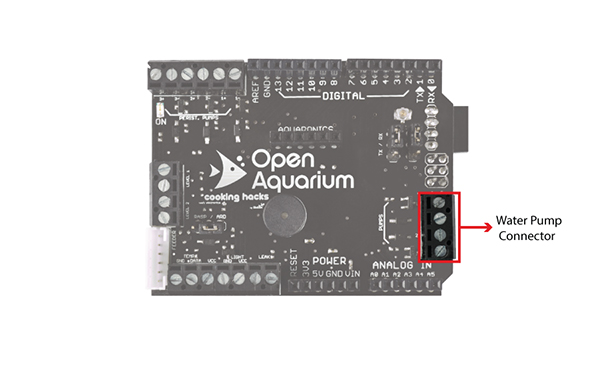
\includegraphics[height=2in]{images/water_pump_connection}
    \caption{Anschluss der Wasserpumpe}
\end{figure} \\
Pumpleistung: 100-350 l/h \\
Spannung: 3.5-12V DC \\
Leistungsbereich: 0.5W-5W \cite{WaterPump}\\
\myparagraph{Option 2: Handelsübliche Aquariumpumpe}
Die Pumpe von cooking-hacks.com ist sehr klein und würde gerade einmal reichen um die Pflanzen mit Wasser zu versorgen. Um aber den Wasserkreislauf des Aquariums (150 Liter) zu regeln, ist sie um einiges zu schwach. \\ \mbox{} \\
Es müsste also eine zusätzliche Pumpe eingebaut werden um diesen Kreislauf zu regulieren. Dadurch wird die Pumpe von cooking-hacks.com redundant, weil sie einfach durch eine Erweiterung des Wasserkreislaufes ersetzt werden kann, sodass das Blumenbeet über einen \gls{NFT}-Kanal mit einbezogen ist. Das Wasser wird also vom Aquarium durch den Filter der Außenpumpe geleitet um anschließend die Pflanzen über den \gls{NFT}-Kanal zu düngen und wieder zurück ins Aquarium zu fließen.\\ \mbox{} \\
Es wurde also einzig und allein auf eine normale (statische) Außenpumpe (JBL Cristalprofi E901 Greenline) gesetzt. Diese ist mit einer Pupmleistung von 900 l/h für das verwendete 120x40x50cm große Aquarium bestens geeignet. \cite{JBL}

\newpage
\subsubsection{Mineralienpumpe}
Bei dieser Pumpe handelt es sich um eine Schlauchpumpe. Eine Schlauchpumpe treibt ein Medium durch, von außen einwirkende Rollen, durch einen Schlauch. Sie ist auf einzelne Tropfen genau und eignet sich deshalb gut um  empfindliche Parameter eines Ökosystems mithilfe von speziellen Lösungen zu regulieren. Es können insgesamt drei Pumpen angeschlossen werden, wobei im Normalfall werden zwei davon an Gefäße mit Flüssigkeiten mit einem pH-Wert von 4 und 10 angehängt werden. \cite{hitec-zang} \\ \mbox{} \\
Wie bei der Wasserpumpe ist der Code zum Aktivieren und Deaktivieren der Pumpe kurz.
\begin{lstlisting} [frame=single, caption=Steuern der Peristaltikpumpe]
OpenAquarium.perpumpON(1); // switch pump nr 1 on
OpenAquarium.perpumpOFF(1); // switch pump nr1 off
\end{lstlisting}
Zum Anschließen der Pumpen sind ebenfalls Steckplätze vorhanden. \\
\begin{figure}[ht]
    \centering
    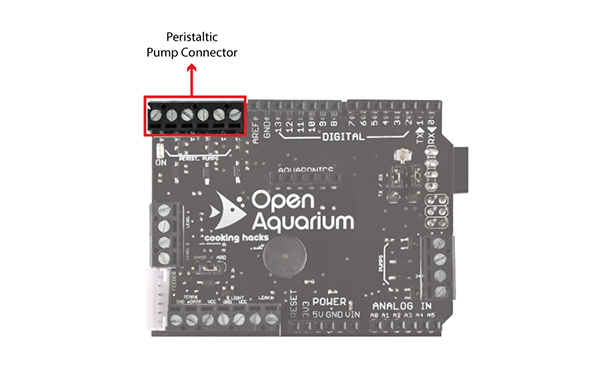
\includegraphics[height=2.1in]{images/mineral_pump_connection}
    \caption{Anschluss der Peristaltikpumpe}
\end{figure} \\
12V DC input voltage \\
Flow: 20-60 ml/min \cite{PeristaltikPump}
\newpage
\myparagraph{Fazit}
Die automatische Regulierung des pH-Wertes sollte nicht auf Dauer (mehr als 2 Monate) verwendet werden, da der pH-Wert Sensor mit der Zeit verschleißt und verfälschte Ergebnisse liefert. Abgesehen davon ist die Regulierung des pH-Wertes auch nur zu Beginn bzw. nach der Besetzung eines Aquaponik-Systems essentiell, da gerade in dieser Zeitspanne der pH-Wert instabil ist.  \\ \mbox{} \\
Da während dem Projekt aus finanziellen Gründen lediglich eine einzige Schlauchpumpe - anstatt der vorgesehenen \textit{drei} - zur Verfügung stand, wurde diese nicht zum Regulieren des pH-Wertes, sondern zum Einspeisen von spezialisierten Minerallösungen in das Aquarium verwendet. \\ \mbox{} \\
Auf Seiten der Software, wären alle Möglichkeiten gegeben, alle drei Pumpen zu implementieren, jedoch konnte aufgrund der Kosten der Pumpen im Rahmen dieses Projektes nur eine der beschriebenen Möglichkeiten umgesetzt werden. 

\newpage
\subsubsection{Futterautomat}
Um den Wartungsaufwand zu minimieren, war ein Futterautomat notwendig, der \"uber eine Weboberfl\"ache konfiguriert werden kann. Es konnte entweder auf einen teuren Futterautomaten gesetzt werden, der diese Option anbietet, oder ein handelsüblicher Futterautomat wird so bearbeitet, dass er als Reaktion auf ein Stromsignal Futter ausgibt. \\
Der Futterautomat von Ponix Systems geh\"ort zur letzteren Art. Sobald 5 Volt angelegt wird, gibt er Futter aus. So kann \"uber die Webapp das Intervall und die Menge gesteuert werden. \\
Da die \gls{GPIO} Pins des Raspberry Pi's allerdings nur 3,3 Volt liefern, musste entweder ein Spannungsteiler verwendet werden, oder ein Transistor, der an 5 Volt angelegt ist und entsprechend durchgeschaltet wird. Da der 5 Volt Ausgang ohnehin nicht gebraucht wird, wird auf die Lösung mit dem Transistor zurückgegriffen. Dafür wird ein "`General Purpos Transistor"' mit einem PNP-Übergang verwendet, welcher in einem Bereich von 0 bis maximal 50 Volt arbeitet und somit für den vorgesehenen Verwendungszweck geeignet ist. \cite{BC557} \\ \mbox{} \\
Die Bezeichnung des Transistors lautet: \texttt{BC557}
\\ \mbox{} \\
Das folgende Script soll beispielhaft zeigen wie der Futterautomat, der nach dem eben beschriebenen Aufbau angeschlossen ist, anzusteuern ist.
\begin{lstlisting}[language=Python]
import RPi.GPIO as GPIO
import time

GPIO.setmode(BOARD)
GPIO.setup(10, GPIO.OUT)

GPIO.output(10, GPIO.HIGH)
time.sleep(5)   # activate for 5 seconds
GPIO.output(10, GPIO.LOW)

GPIO.cleanup()
\end{lstlisting}
\newpage
Der Schaltplan für den beispielhaften Code sieht demnach wie folgt aus: \\ \mbox{} \\
\begin{figure}[ht]
    \centering
    \includegraphics[width=12cm]{images/fishFeeder}
    \caption{Schaltplan für den Futterautomaten}
\end{figure}
\newpage
\subsubsection{Pflanzenbeleuchtung}
\myparagraph{Option 1: Cooking Hacks}
Die Beleuchtung könnte mit einem \gls{LED} Streifen (www.cooking-hacks.com) realisiert werden. Er besteht aus 72 LEDs (60 Weiße und 12 Blaue) mit einer Leuchtkraft von 500 Lumen. Der Streifen kann mit Hilfe der OpenAquarium Klasse der aktuellen Zeit automatisch angepasst werden. Der folgende Code, steuert die Lampe so, dass sie für die Pflanze eine Sonne simuliert.
\begin{lstlisting} [language=C, caption=Steuerung des LED-Streifens von cooking-hacks]
now = OpenAquarium.getTime();
OpenAquarium.printTime(now);
OpenAquarium.lighting(now);
\end{lstlisting}
Wie bei den beiden Pumpen kann der \gls{LED} Streifen am OpenAquarium Board angeschlossen werden. \\
\begin{figure}[ht]
  \centering
    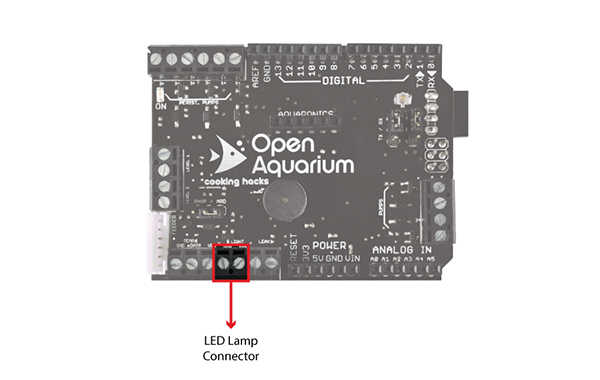
\includegraphics[height=1.8in]{images/led_connection}
    \caption{Anschluss der Beleuchtung}
\end{figure} \\
Leistung: 5.5 watts \\
Beleuchtung: 72 \gls{LED}s \\
Farbe: 60 Weiße + 12 Blaue \cite{LEDLamp}\\

\newpage
\myparagraph{Option 2: Eigenbau von Ponix Systems}
Als Alternative wird ein LED-Brett von Ponix Systems zur Verfügung gestellt. Dieser hat die Fähigkeit einige, für Pflanzen, wichtige Lichtspektren auszustrahlen. Es benötigt eine Stromversorgung mit 24 Volt und ein pulsierendes Signal auf dem EN-Eingang. Dieses Signal wird verwendet um die Intensität des Lichtes zu steuern, indem eine gewisse Frequenz vom Raspberry Pi gesendet wird. Dazu wird ein so genannter \gls{PWM}-Pin (Pulsweitenmodulation) verwendet. Aus Erfahrungswerten der Firma Ponix Systems, ist diese Lösung deutlich besser für die Wachstumsdauer der Pflanzen. \cite{osram, elektrJournal} \\ \mbox{} \\
Die LED-Bretter haben jeweils drei Eingänge: +, -, EN \\
Es wird also auf die Lösung von Ponix Systems zurückgegriffen, welche einen höheren Programmieraufwand erfordert, dafür allerdings einen großen Vorteil für die Pflanzen. Die Qualität könnte immer noch durch besser spezialisierte Beleuchtung weiter verbessert werden (Siehe 8.1.3). 
\begin{figure}[ht]
    \centering
    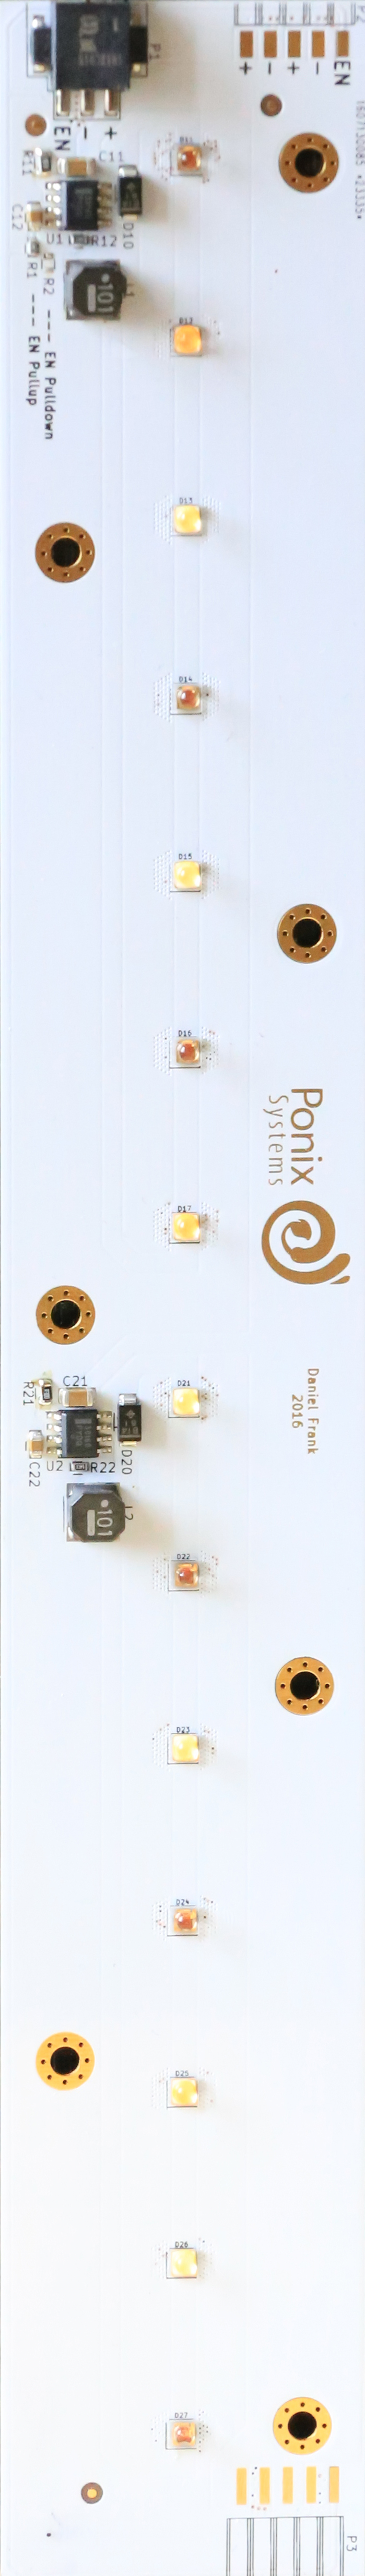
\includegraphics[angle=90, width=15cm]{images/pflanzenLicht}
    \caption{Lichtstreifen von Ponix Systems}
\end{figure} \\ \mbox{} \\
Der Aufbau der Schaltung sieht demnach wie folgt aus: \\
\begin{figure}[ht]
    \centering
    \includegraphics[height=8cm]{images/LED-Brett-Anschluss}
    \caption{Schaltung für LED-Bretter}
\end{figure} 
\newpage
Wenn die Pflanzenbeleuchtung nach der eben gezeigten Schaltung aufgebaut ist, kann die Intensität mithilfe der Frequenzregulierung des PWM-Pins gesteuert werden. Im folgenden Beispielcode wird das LED-Brett für eine Stunde mit einer Intensität von 50 Prozent aktiviert.
\begin{lstlisting}[language=Python, caption=Steuern der Pflanzenbeleuchtung]
import RPi.GPIO as GPIO
import time

GPIO.setmode(GPIO.BOARD)
GPIO.setup(12, GPIO.OUT)
light = GPIO.PWM(12, 100)
light.start(50)  # start with intensity of 50 percent
time.sleep(3600) # expose for 1 hour
light.ChangeDutyCycle(0) # set intensity to 0

GPIO.cleanup()
\end{lstlisting}

\newpage
\subsubsection{Hitzestrahler}
Es gibt für das OpenAquarium Board keinen Hitzestrahler der entsprechend konfiguriert werden und eine bestimmte Temperatur halten kann. \\ \mbox{} \\
\begin{figure}[ht]
  \centering
  \includegraphics[height=2.2in]{images/heaterPipePlan}
  \caption{Schaltplan zum Steuern des Hitzestrahlers}
\end{figure} \mbox{} \\ \mbox{} \\
Am benutzerfreundlichsten erschien es den Hitzestrahler auf die höchstmögliche Temperatur einzustellen und je nach aktueller Temperatur, und der vom Benutzer über die Webapp angegebenen Wunschtemperatur, des Aquariums, das Relais zu aktivieren bzw. zu deaktivieren. \\ \mbox{} \\
Das Problem beim Steuern des Hitzestrahlers über das Internet ist, dass einige Störfak-toren einwirken. Daten könnten geändert/gefälscht werden, der Sensor könnte falsche Daten liefern, das Relais könnte eine Fehlfunktion aufweisen. Wenn eine dieser Fälle eintritt, wird das Aquarium so warm, dass sämtliche Fische sterben würden. Daher ist es sinnvoller den Hitzestrahler nicht über das Netzwerk zu steuern, sondern manuell einzurichten. Der Benutzer muss also lokal, den Hitzestrahler an seine Bedürfnisse anpassen. 
\newpage
%%%%%%%%%%%%%%%%%%%%%%%%%%%%%%%%%%%%
%               LED                %
%%%%%%%%%%%%%%%%%%%%%%%%%%%%%%%%%%%%
\subsubsection{RGB-LED-Streifen}
Um das Aquarium von innen heraus zu beleuchten, werden wasserdichte \gls{RGB}-\gls{LED}-Streifen verbaut. Dabei soll die Intensität der einzelnen Farben (Rot, Grün und Blau) über die Webapp angepasst werden können, um so die gesamte Farbe zu regulieren. Um dies zu ermöglichen, wurden die einzelnen Kanäle über eine Schaltung mit dem Raspberry Pi verbunden. Diese Schaltung besteht aus drei MOSFET's, die jeweils einen Farbkanal übernehmen, wie in der Graphik auf der folgenden Seite zu sehen ist (Abbildung 12). \\ \mbox{} \\
Um eine bestimmte Farbe zu aktivieren, wird das Programm und Python Library \texttt{pigpio} verwendet. Mit der Kommandozeile kann beispielsweise die Farbe "`Karminrot"' - rgb(161, 35, 43) - mit folgendem Befehl eingerichtet werden:
\begin{center}
    \texttt{sudo pigpiod pigs p 40 161 pigs p 38 35 pigs p 38 43}
\end{center} \mbox{} \\
Konkret wird mit diesem Kommando gleichzeitig der \texttt{pigpiod}-Daemon gestartet und Parameter für die Steuerung der Pins übergeben. Der Daemon kann zur Laufzeit GPIO-Pins steuern, indem Nachrichten an ihn gesendet werden. Diesen Teil übernimmt \texttt{pigs}. Mit \texttt{pigs} wird die Pulsweitenmodulation eines GPIO-Pins angepasst und aktualisiert. Mit Hilfe dieser Frequenz und der verbauten Schaltung (Abbildung 9) können die einzelnen Farben (Rot, Grün und Blau) einzeln gesteuert werden.
\begin{figure}[ht]
    \centering
    \includegraphics[width=7cm]{images/pigs.png}
    \caption{Syntax von pigs}
\end{figure}
\begin{figure}[hp]
    \centering
    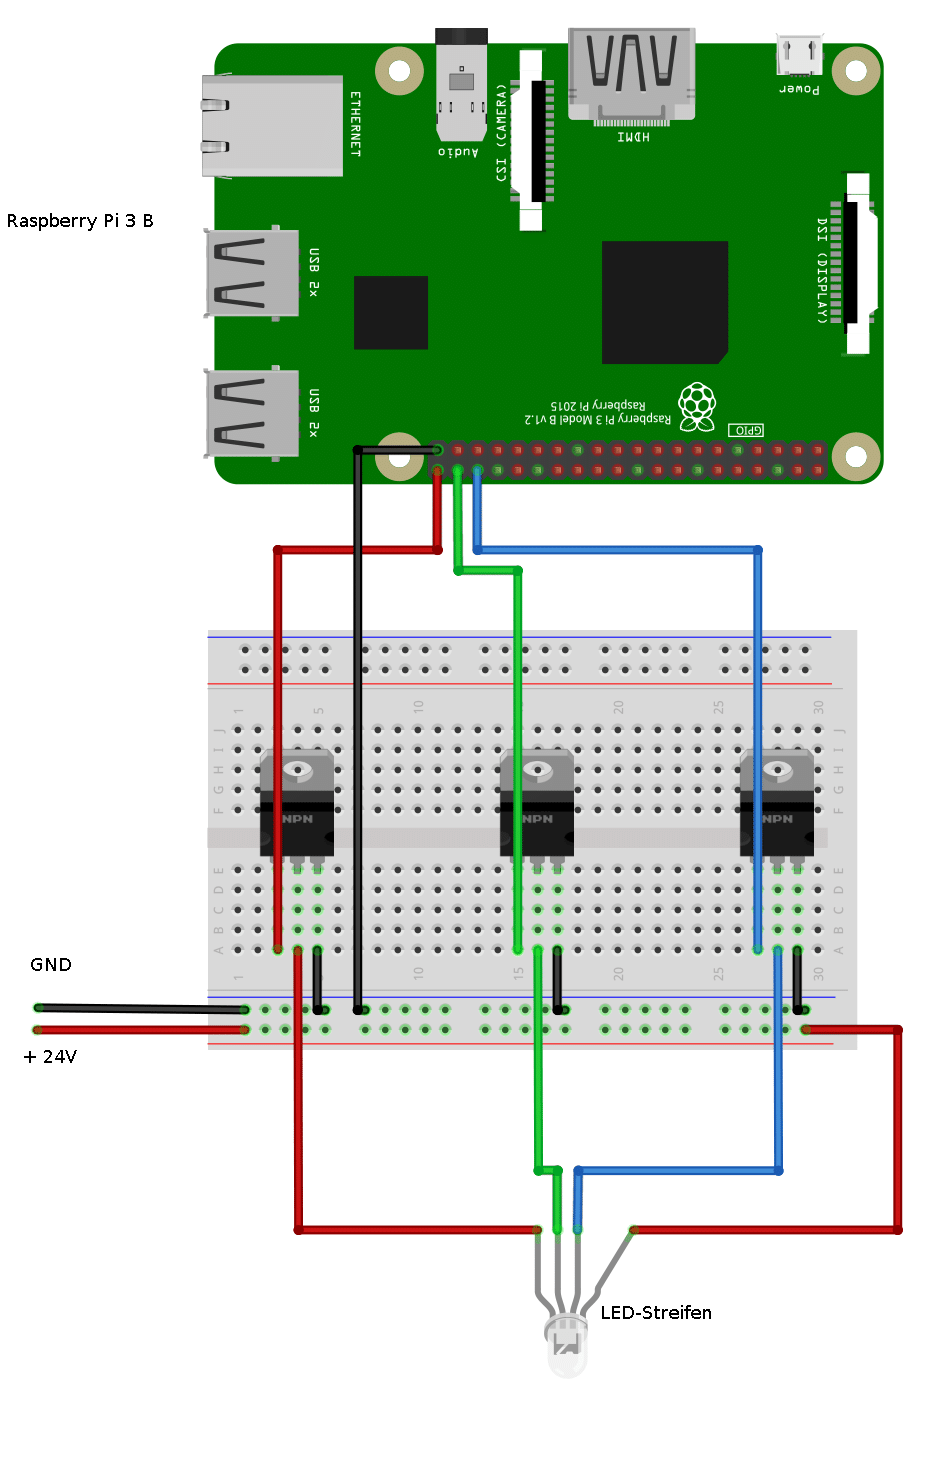
\includegraphics[width=13cm]{images/led_stripe}
    \caption{RGB-LED-Streifen Schaltplan}
\end{figure}

\newpage
%%%%%%%%%%%%%%%%%%%%%%%%%%%%%%%%%%%%%
%             Sensoren              %
%%%%%%%%%%%%%%%%%%%%%%%%%%%%%%%%%%%%%
\subsection{Sensoren}
Die Sensoren f\"ur den Prototypen, werden von der Firma Ponix Systems zur Verf\"ugung gestellt. Diese mussten allerdings erst auf Funktionalit\"at untersucht werden. \\
F\"ur die Entwicklung, des Codes, zum Ansprechen der Sensoren, wird "`Arduino \gls{IDE}"' verwendet. Diese \gls{IDE} bietet die M\"oglichkeit, den Code auf einem rechenstarken PC zu kompilieren und ihn dann auf dem Arduino auszuf\"uhren. Zus\"atzlich kann sie verwendet werden, um alle eingehenden Daten des Arduinos zu \"uberwachen.
Der kompilierte Code wird beim Endprodukt auf dem Arduino gespeichert und sendet kontinuierlich Daten \"uber die \gls{USB} Schnittstelle an den Raspberry Pi. Es werden Libraries von Arduino indirekt \"uber die \gls{API} von OpenAquarium verwendet. \\ \mbox{} \\
Alle folgenden Abbildungen, die die Anschlussmöglichkeiten der Sensoren und Aktoren beschreiben,wurden von cooking-hacks übernommen. \cite{OpenAquarium}

\newpage
\subsubsection{Temperatur}
Zum Messen der Temperatur wird der Sensor von www.cooking-hacks.com verwendet (DS18B20): \\
Input: 3.0-5.5V  \\
Arbeitsbereich: -55\degree C bis +125\degree C  \\
Genauigkeit: $\pm$ 0.5\degree C von -10\degree C bis +85\degree C \cite{TempSensor} \\
\mbox{}\\
Die Temperatur kann mit nur einem Befehl abgelesen werden. Dieser liefert einen Wert in Grad Celsius zur\"uck.
\begin{lstlisting} [language=C, caption=Auslesen der Temperatur]
OpenAquarium.init();
float temperature = OpenAquarium.readtemperature();
\end{lstlisting}
Die Testergebnisse des Temperatur Sensors stimmten mit den Werten eines handelsüblichen Thermometers überein.  \mbox{} \\
Angeschlossen werden die Sensoren bzw. der Temperatursensor auf dem OpenAquarium Board: \\
\begin{figure}[ht]
	\captionsetup{justification=raggedright}  
	\begin{minipage}[b]{.4\textwidth}  
		\centering  
		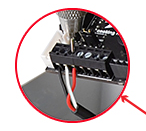
\includegraphics[width=3.5cm]{images/temp_sensor_connection_detail}  
	\end{minipage}%  
	\begin{minipage}[b]{0.6\textwidth}  
		\centering  
		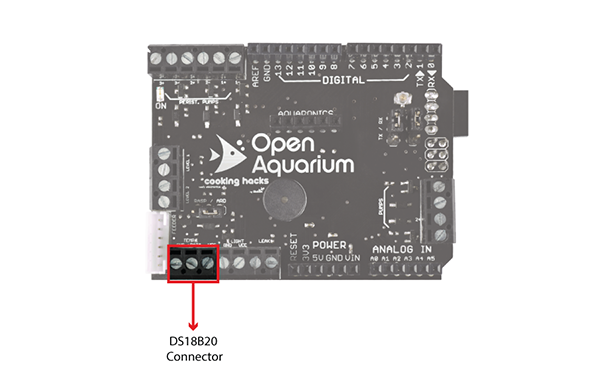
\includegraphics[width=8cm]{images/temp_sensor_connection}  
	\end{minipage}
	\par
	\begin{minipage}[t]{.4\textwidth}
		\centering  
		\caption{Detaillierte Darstellung der Anordnung der Kabel vom Temperatursensor}  
	\end{minipage}%
	\begin{minipage}[t]{.6\textwidth}  
		\centering  
		\caption{Anschluss des Temperatursensors}  
	\end{minipage}  
\end{figure}

\newpage
\subsubsection{EC Wert}
Der \gls{EC} Wert (Electrical Conductivity) gibt über die Leitfähigkeit des Wassers Auskunft. Mit diesem Wert kann grob auf die Menge der im Wasser gelösten Minerale/Salze geschlossen werden. Desto mehr N\"ahrstoffe im Wasser vorhanden sind, desto h\"oher ist auch der \gls{EC} Wert. \\ \mbox{} \\
Angeschlossen wird der Sensor auf dem OpenAquarium Board: \\
\begin{figure}[ht]
    \centering
    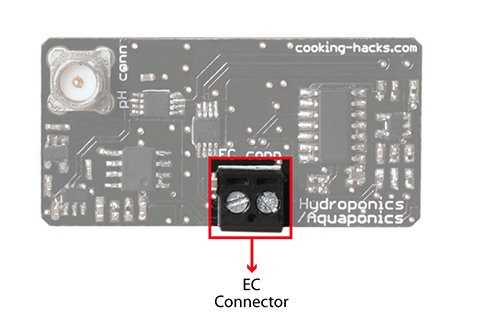
\includegraphics[height=2.0in]{images/ec_sensor_connection}
    \caption{Anschluss des \gls{EC}-Sensors}
\end{figure}

Um den EC Wert zu messen wird der Sensor von www.cooking-hacks.com verwendet, welcher mit folgendem Code angesprochen werden kann: \cite{TempSensor}

\begin{lstlisting} [frame=single, caption=Auslesen des EC Wertes]
OpenAquarium.init();
OpenAquarium.calibrateEC(point_1_cond,point_1_cal,
                         point_2_cond,point_2_cal);

float resistanceEC = OpenAquarium.readResistanceEC();
float EC = OpenAquarium.ECConversion(resistanceEC); //EC Value in uS/cm
\end{lstlisting}
\newpage
Die Tests beim Eintauchen des Sensors in Leitungswasser ergaben folgende Ergebnisse: \\
\begin{figure}[ht]
    \centering
    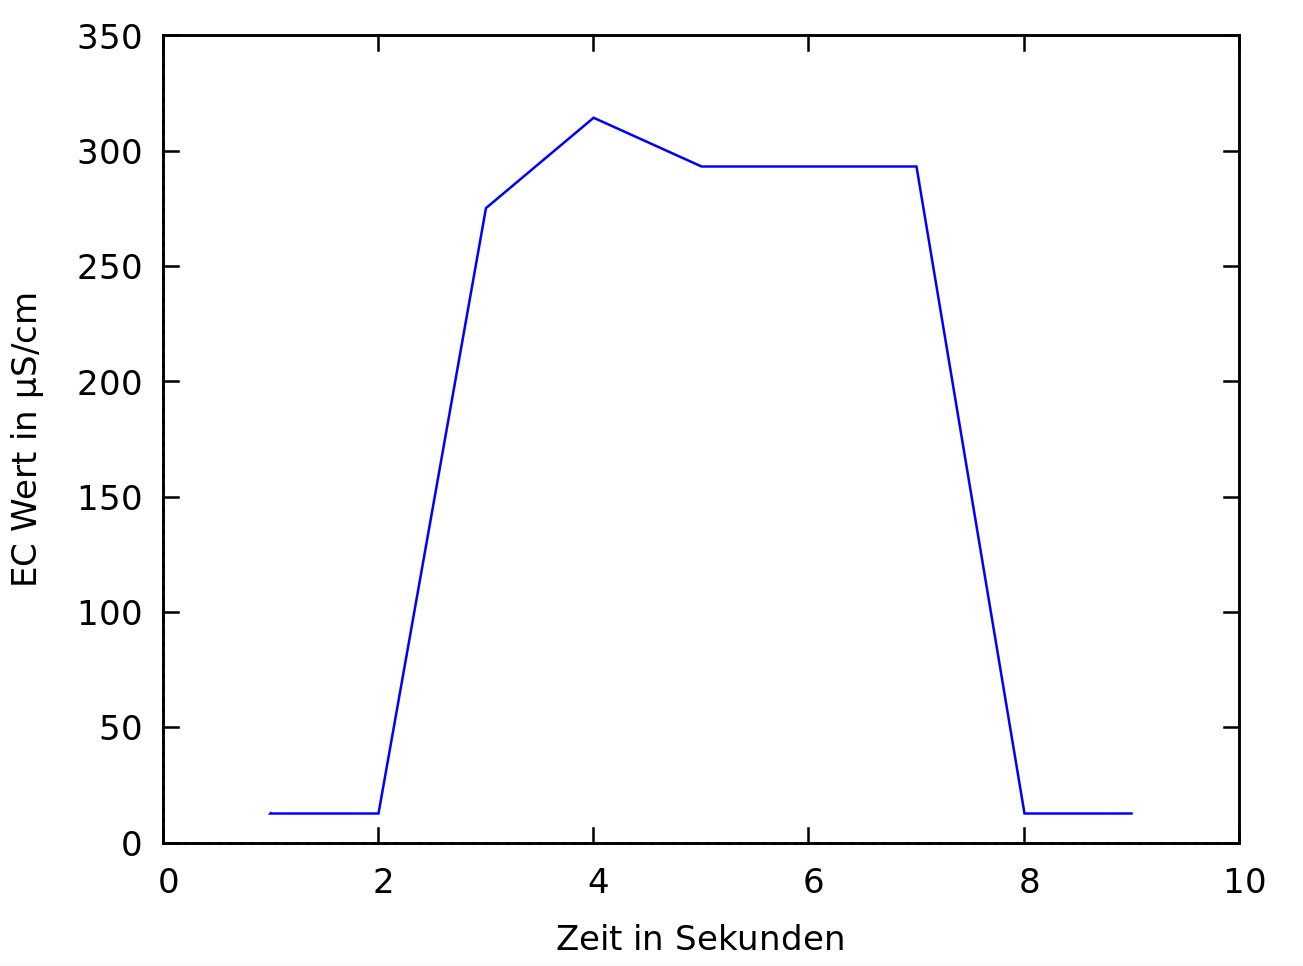
\includegraphics[height=3.2in]{images/ec_tests}
    \caption{Testergebnisse des EC-Sensors}
\end{figure}

\vskip0.5cm \mbox{} \\
Wie erwartet, steigt der \gls{EC} Wert beim Eintauchen ins Wasser, da es nat\"urlich um einiges leitf\"ahiger ist, als Luft. \\ \mbox{} \\

\newpage

\subsubsection{pH Wert}
Der pH-Wert ist einer der wichtigsten Werte, wenn es um das \"Uberwachen eines Aquaponik Systems geht. Es gibt ein gro{\ss}es Spektrum an erh\"altlichen Sensoren. Die der unteren Preisklasse, ben\"otigen regelm\"a{\ss}ige Wartungen, während die der oberen Preisklasse den Preis des Produktes, \"uber die Zielgruppe hinaus heben und somit unbrauchbar sind. Weil der Preis einer der ausschlaggebensten Punkte vom Homeponics System ist, musste auf einen billigen Sensor von www.cooking-hacks.com zurückgegriffen werden. Da allerdings die Überwachung des pH-Wertes gerade beim Besetzen eines Aquaponik Systems essentiell ist und danach nur noch gelegentlich geprüft werden muss, ist die Wartung nur zu Beginn von großer Bedeutung. Danach können je nach Stabilität des Ökosystems Wartungen ausgelassen werden. Da der Sensor ein analoges Signal liefert, muss die gemessene Spannung erst umgerechnet werden. Diese Aufgabe \"ubernimmt die Klasse OpenAquarium der OpenAquarium-Library für den Arduino (Siehe 4.2). \cite{pHsensor, abcChemie} \\

\begin{lstlisting} [frame=single, caption=Auslesen des pH-Wertes]
OpenAquarium.calibratepH(cp4,cp7,cp10);
int mvpH = OpenAquarium.readpH(); //Value in mV of pH
float pH = OpenAquarium.pHConversion(mvpH);
\end{lstlisting}
cp4, cp7, cp7 ... Calibrationpoints (Konstanten)

\paragraph{Calibrationpoints} \mbox{} \\
Zu den Calibrationpoints (Kalibrierungswerte) ist zu erwähnen, dass sie angepasst werden, wenn der gemessene pH-Wert zu stark vom eigentlichen Wert abweicht. Um die Abweichung des Sensors zu beheben, sind Kalibrierungskits vorgesehen, die allerdings bis zu ein mal im Monat verwendet werden m\"ussen. \\ \mbox{} \\
\newpage 
Angeschlossen wird der Sensor auf dem OpenAquarium Board. \\
\begin{figure}[ht]
    \centering
    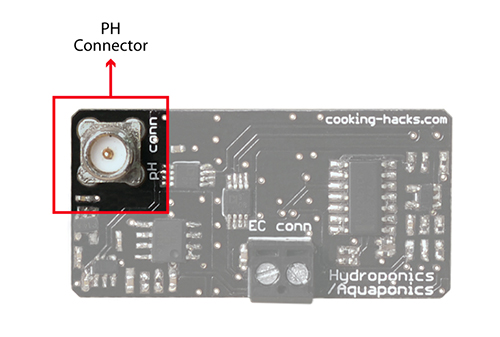
\includegraphics[height=2.0in]{images/ph_sensor_connection}
    \caption{Anschluss des pH-Sensors}
\end{figure}

\paragraph{Tests} \mbox{} \\
Beim Testen eines bereits l\"anger in Betrieb (2 Monate) gewesenem pH-Sensor brachte dieser folgende Ergebnisse: \\
\begin{figure}[ht]
    \centering
    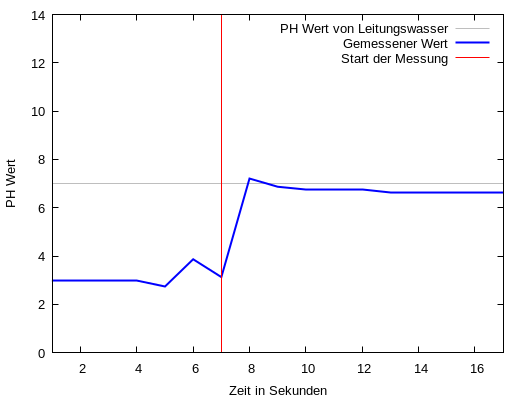
\includegraphics[height=2.7in]{images/ph_tests}
    \caption{Testergebnisse des pH-Sensors}
\end{figure} \\
Wie zu sehen ist, weicht der gemessene Wert bereits stark (0.5) von dem eigentlichen Wert ab. Für empfindliche Fische ist eine pH-Wertabweichung in diesem Ausmaß bereits tödlich. Ein Beispiel dafür, ist der Blaue Neon, dessen Lebensbereich zwischen einem pH-Wert von 5,5 und 6 eingegränzt ist, während die Guppies für ihre Robustheit von 6 - 8,5 beliebt sind. 
\paragraph{Fazit} \mbox{} \\
Da es keine pH-Sensoren gibt, die billig sind und zugleich einen niedrigen Wartungsauf-wand aufweisen, könnte eine eigene Lösung zur pH-Wert-Messung, wie etwa eine Auswertung eines Teststreifens mittels einer Kamera, eingebaut werden. Da diese Eigenbaulösungen den Arbeitsaufwand überschreiten würden und nur mit beschränkter Aussicht auf Erfolg zu beurteilen sind, wird weiterhin auf die billigere Variante gesetzt und in Kauf genommen, dass der Benutzer hin und wieder Wartungsarbeiten erledigen muss. Dieser Lösungsweg ist zusätzlich vertretbar, da der pH-Wert Sensor gerade am Anfang der Bestückung eines Aquaponik Systems von großer Bedeutung ist. Ohne ihn müssten einige Teststreifen verwendet werden, wohingegen die Daten des pH-Sensors sich nur allmählich mit der Zeit verfälschen.
\newpage

\newpage
%%%%%%%%%%%%%%%%%%%%%%%%%%%%%%%%%%%%%
%               DBMS                %
%%%%%%%%%%%%%%%%%%%%%%%%%%%%%%%%%%%%%
\subsection{Datenbankmanagementsystem}
\cfoot{Konrad Kelc}
In diesem Kapitel werden verschiedene Datenbanksysteme, die für das Projekt in Frage kommen analysiert und auf ihre Tauglichkeit hin überprüft.
\subsubsection{\gls{RDBMS} vs. \gls{NoSQL}}
Zur Speicherung der Sensordaten soll ein geeignetes Datenbankmanagementsystem verwendet werden. Zu Beginn wird evaluiert, ob ein relationales oder ein \gls{NoSQL}-Datenbank-system verwendet wird. Dabei werden die jeweiligen Vor- und Nachteile von \gls{SQL} und \gls{NoSQL} Datenbanken aufgelistet. Auf Performance, Konsistenz und den einfachen Zugriff auf Daten, wird dabei besonders Wert gelegt.

Folgend werden alle Kriterien kurz aufgeschlüsselt definiert.

\begin{itemize}
	\item \textbf{Performance:} \\Gibt an, wie schnell die Lese- und Schreibleistung ist.
	\item \textbf{Konsistenz:} \\Gibt an, wie gut das \gls{DBMS} Ma{\ss}nahmen zur Konsistenzerhaltung umsetzt.
	\item \textbf{einfacher Zugriff auf Daten:} \\Gibt an, wie Umfangreich die \gls{API} des \gls{DBMS} ist.
\end{itemize}

Die Abfragesprache SQL wir auf die drei Teile \gls{DDL} (Data Definition Language), \gls{DML} (Data Manipulation Language) und \gls{DCL} (Data Control Language) aufgeteilt.

\begin{itemize}
	\item \textbf{\gls{DDL}}:\\ ist die Sprache f\"ur das Anlegen, \"Andern und L\"oschen von Datenstrukturen.
	\item \textbf{\gls{DML}}:\\ ist die Sprache f\"ur das Abfragen, Einf\"ugen, \"Andern oder L\"oschen von Nutzdaten.
	\item \textbf{\gls{DCL}}:\\ ist die Sprache f\"ur die Zugriffskontrolle.
\end{itemize}

\newpage

\textbf{Konsistenz}\\\\
\gls{SQL}-Datenbanken verwenden das \gls{ACID} Prinzip, daher besitzen sie eine bessere Konsistenz als
\gls{NoSQL}-Datenbanken. \gls{NoSQL} Datenbanken verwenden das \gls{BASE} Prinzip, die Daten hier sind daher
nur "`schlussendlich"' konsistent. Dadurch kann es passieren, dass nach einem Update nicht immer
dieselben Werte zur\"uckgeliefert werden, die vor dem Update bereits vorhanden waren. Jedoch besitzen sie wegen ihres einfachen Schemas und trotz hohen Datenvolumens, eine hohe Skalierbarkeit.

Zusammenfassend kann gesagt werden, das \gls{SQL}-Datenbanken eine bessere Konsistenz aufweisen, aber \gls{NoSQL}-Datenbanken eine bessere Performance und Skalierbarkeit besitzen. Da wir besonderen Wert auf die Performance
legen, haben wir uns entschieden für das Projekt eine \gls{NoSQL}-Datenbank zu verwenden.

Im Bezug auf das \gls{NoSQL}-Datenbanksystem waren folgende Kriterien von Bedeutung:

\begin{itemize}
	\item \textbf{Performance:} \\Gibt an, wie schnell die Lese- und Schreibleistung ist.
	\item \textbf{einfacher Zugriff auf Daten:} \\Gibt an, wie Umfangreich die API des DBMS ist.
	\item \textbf{Dokumentation:}\\ Gibt an, wie gut das \gls{DBMS} dokumentiert ist.
	\item \textbf{Verbreitung:}\\ Gibt an, wie weit das \gls{DBMS} verbreitet ist.
\end{itemize}

Die Folgenden \gls{NoSQL} Datebankmanagementsysteme wurden evaluiert:

\begin{itemize}
	\item MongoDB
	\item Redis
\end{itemize}

\subsubsection{MongoDB}
\label{sec:mongoDB}
MongoDB ist eine schemafreie, dokumentenorientierte NoSQL-Datenbank, die in der Programmiersprache C++ geschrieben ist. Da die Datenbank dokumentenorientiert ist, kann sie Sammlungen von \gls{JSON}-\"ahnlichen Dokumenten verwalten. So k\"onnen viele Anwendungen Daten auf nat\"urlichere Weise modellieren, da die Daten zwar in komplexen Hierarchien verschachtelt werden k\"onnen, dabei aber immer abfragbar und indizierbar bleiben. Au{\ss}erdem ist MongoDB eine Allzweckdatenbank mit offenem Quellcode (OpenSource). \cite{MongoDB_wiki}

\newpage
Sie hat u.a. folgende Merkmale: \cite{MongoDB_characteristics}

\begin{itemize}
	\item Dokumentdatenmodell mit dynamischen Schemata
	\item Umfassende, flexible Indexunterst\"utzung
	\item Aggregation-Framework und MapReduce
	\item Auto-Sharding f\"ur horizontale Skalierbarkeit
	\item Eingebaute Replikation f\"ur Hochverf\"ugbarkeit
	\item Textsuche
	\item Erweiterte Sicherheit (z.B. Kerberos Unterst\"utzung)
	\item Speicherung gro{\ss}er Dateien mit GridFS
\end{itemize}

\subsubsection{Redis}
Im Vergleich dazu ist Redis eine In-Memory-Datenbank mit einer einfachen Schl\"ussel-Werte-Datenstruktur. Nach einer Erhebung von DB-Engines.com ist Redis der verbreitetste Schl\"ussel-Werte-Speicher. \cite{db-engines}\\
Die einfache Struktur der Datenbank eignet sich weniger f\"ur komplexe Datenstrukturen, die \"uberwiegend in der Datenbank selbst abgebildet werden soll, daf\"ur ist der gro{\ss}e Vorteil von Redis, dass es schneller ist als relationale Datenbanken wie z.B. \gls{MySQL}. Wie ein Benchmark auf einem alten Macbook (2.66 GHz Intel Core 2 Duo) gezeigt hat, sind Lese- und Schreibperformance nahezu gleich auf.  Mit jeweils ca 37000 Zugriffen pro Sekunde beweist das schwache Notebook die hohe Performance von Redis. \cite{redisBenchmark}\\
Redis bietet Persistenz durch automatisiertes regelm\"a{\ss}iges Abspeichern oder per Protokolldatei, wodurch bei entsprechender Konfiguration auch eine \gls{ACID}-konforme Dauerhaftigkeit erreichbar ist. \cite{Redis_Evaluation}

Zusammenfassend kann man sagen dass, Redis bei den Kriterien, wie z.B. der Performance und den einfachen Zugriff auf Daten durch
seine Kompaktheit, besser abschneidet, jedoch den gro{\ss}en Nachteil hat, dass es bei serverseitiger Verwendung, extrem viel Arbeitsspeicher verbraucht, wenn einige Homeponics Systeme ihre Daten \"uber den Server persistieren.

\subsubsection{Fazit}
Es m\"ussen sowohl auf dem lokalen Raspberry Pi, als auch auf dem Server Echtzeitdaten vorhanden sein, um einerseits auf dem Touchdisplay eine \"Ubersicht anzuzeigen und andererseits \"uber den Browser alle Daten zu betrachten. Da auf dem Raspberry Pi genügend Arbeitsspeicher vorhanden ist um die aktuellen Daten zwischenzuspeichern eignet sich Redis am besten für diese Aufgabe.
\newpage

%%%%%%%%%%%%%%%%%%%%%%%%%%%%%%%%%%%%%
%           Web Framework           %
%%%%%%%%%%%%%%%%%%%%%%%%%%%%%%%%%%%%%
\subsection{Web Framework}
\cfoot{Ramin Bahadoorifar}
Bei Web Frameworks, werden durch vordefinierte und vorgefertigte Klassen, h\"aufig gebrauchte Funktionen wie Mailversand, sichere Authentifizierung, Sicherheitsfunktionen, Lokalisierung, Performance (z.B. \gls{HTTP} Caching) oder grundlegende Funktionen f\"ur Webformulare vereinfacht. \\
Web Frameworks sind darauf ausgelegt, sehr schnell Ergebnisse zu erzielen und lauff\"ahige Webanwendungen zu erstellen. Dazu bieten sie einen Datenbankzugriff, Templating-Mechanismen, eine saubere Trennung von Pr\"asentation und Code durch Verwendung des \gls{MVC}-Prinzipes. \\
Da eine eigenst\"andige Implementierung all dieser Mechanismen den Arbeitsaufwand \"ubersteigen w\"urde, ist eine Verwendung eines solchen Web Frameworks unabdinglich. Welches Framework dabei gew\"ahlt wird h\"angt von folgenden Komponenten ab:
\begin{itemize}
\item Schwierigkeitsgrad
\item Lernkurve
\item Sicherheit
\item Dokumentation
\end{itemize}
\newpage
\subsubsection{Django}
Django ist ein in Python geschriebenes opensource Web Application Framework, das dem Model-View-Presenter-Schema folgt.
\paragraph{Schwierigkeitsgrad/Lernkurve} \mbox{}\\
Da Python selbst leicht zu erlernen ist, ist es keine Herausforderung sich in die Sprache einzuarbeiten. Das Framework ansich, gilt als eines der einfachereren (aber auch funktionsarmeren) seiner Art und bietet daher eine flache Lernkurve. F\"ur jemanden der bereits mit Webframeworks gearbeitet hat, ist Django schnell zu erlernen.
\paragraph{Sicherheit} \mbox{}\\
Django ist so konzipiert, dass die standartm\"a{\ss}ig implementierten Sicherheitsma{\ss}nahmen, f\"ur den gr\"o{\ss}ten Bereich der Webentwicklung ausreicht. Da zwischen dem Raspberry Pi und dem Server wenig sicherheitsrelevante Daten ausgetauscht werden, gen\"ugt die Sicherheit von Django. \cite{DjangoSecurity}
\paragraph{Dokumentation} \mbox{}\\
Die Dokumentation von Django ist gerade f\"ur Einsteiger optimal, da sie einige n\"utzliche Tutorials bietet. Aber auch f\"ur erfahrene Entwickler ist die Dokumentation gro{\ss}artig. \cite{DjangoDoc}
\newpage

\subsubsection{Node.js}
Node.js ist eine Event-basierte Plattform, welche nicht blockierend ist. Das bedeutet, dass der Server nicht wartet bis ein Ereignis vollendet wurde, um mit den n\"achsten Aufgaben fortfahren zu k\"onnen. Stattdessen werden Callbacks verwendet, welche dann erst aufgerufen werden, wenn ein bestimmtes Ereignis fertig ausgef\"uhrt wurde, bei dem von einer l\"angeren Dauer ausgegangen wird. W\"ahrenddessen kann der Server andere Aufgaben bearbeiten.\cite{node_eval}

An sich l\"auft Node.js nicht Multi-Threaded, wie man vielleicht erwartet, sondern bearbeitet jede eingehende Verbindung mit einem Thread. Jedoch werden bestimmte Funktionen, wie das Auslesen einer Datenbank oder das Rendern von Templates, intern durch mehrere Threads erledigt, welche dann bei Vollendung den zugewiesenen Callback aufrufen. Durch diese Architektur ist Node.js in vielen Bereichen viel schneller als andere Webserver, die f\"ur jede Verbindung einen Prozess erstellen w\"urden.

Node.js ist sehr abh\"angig durch Third-Party Module, welche durch \gls{NPM} (Node Package Manager) verwaltet und installiert werden k\"onnen. Diese Module machen das Entwickeln von Applikationen viel einfacher oder geben auch mehr Funktionen. F\"ur uns interessante Module w\"aren zum Beispiel: Express.js oder Socket.io. Ersteres gibt uns die M\"oglichkeit die Applikation im \gls{MVC}-Pattern zu entwickeln.
Mit Socket.io k\"onnte man Daten dem Client senden und gleichzeitig empfangen, ohne dabei davor eine Anfrage vom Client erwarten zu m\"ussen. Es gen\"ugt damit nur noch eine Anfrage vom Client bei dem eine Verbindung (Socket) zum Server ge\"offnet wird, sodass man Daten bidirektional senden kann.

\paragraph{Schwierigkeitsgrad/Lernkurve} \mbox{}\\
Wie der Name schon verr\"at verwendet Node.js JavaScript als Programmiersprache. Falls man die Sprache schon kann, wie in unserem Fall, ist eine Lernkurve jeweils in den einzeln verwendeten Modulen sichtbar, die sehr unterschiedlich sind. Somit ist der Schwierigkeitsgrad nicht wirklich einsch\"atzbar. Der Schwierigkeitsgrad in den oben genannten Modulen liegt im mittleren Bereich.

\paragraph{Sicherheit} \mbox{}\\
Node.js hat eine relativ gro{\ss}e Community. Das ist insofern wichtig, da Sicherheitsl\"ucken dadurch schneller gefunden und behoben werden k\"onnen. Jedoch unterscheidet sich die Sicherheit auch in diesem Punkt in den einzelnen Modulen. Somit muss beachtet werden, dass der zu verwendende Modul eine hohe Bekanntheit hat.

\paragraph{Dokumentation} \mbox{}\\
Node.js ist an sich sehr gut dokumentiert und bietet durch eine Vielzahl von Tutorials einen einfachen Einstieg. Von den bekannten Modulen, wissen wir, dass die Dokumentation sehr gut ist, wie bei Socket.io oder Express.js. Au{\ss}erdem wird der Einstieg in diesen Modulen mit verschiedenen Tutorials, die im Internet zu finden sind, sehr einfach gemacht.

\subsubsection{Laravel}
Laravel ist ein \gls{PHP}-Framework und wird von vielen Entwickler derzeit als eines der besten Frameworks f\"ur \gls{PHP} bezeichnet.
Laravel bietet viele Funktionen an, wie Routing, Templating, Unit Testing, usw.

Die Architektur von \gls{PHP} unterscheidet sich von Node.js sehr stark:\cite{php_eval}
\begin{itemize}
    \item Pro Verbindung wird ein neuer Prozess erstellt. Dies hat bei hoher Nutzzahl zur Folge, dass der Arbeitsspeicher des Servers sehr schnell voll werden kann.
    Node.js verwendet nur einen Thread und erstellt, falls erforderlich, mehrere Threads f\"ur eine jeweilige Aufgabe, welche dann bei erfolgreicher Ausf\"uhrung (also Aufrufen des Callbacks) beendet werden. Wird aber ein Fehler hervorgerufen st\"urzt Node.js komplett ab, wogegen bei \gls{PHP} nur der Prozess abst\"urzt.
    \item Jedesmal, wenn ein \gls{PHP}-Skript ausgef\"uhrt wird, wird das Skript neu interpretiert. Dies hat den Vorteil, dass bei einer Code\"anderung nicht der Server neugestartet werden muss. Der Nachteil liegt jedoch in der Performance.
    Bei Node.js wird der Code beim Starten kompiliert. Eine Code\"anderung wirkt sich jedoch solange nicht am Server aus bis Node.js neugestartet wurde. Dies dauert deutlich l\"anger als ein \gls{PHP}-Server. Dagegen ist die Performance in der Laufzeit deutlich schneller als bei \gls{PHP}.
    \item Der Code in \gls{PHP} l\"auft, anders als in Node.js, synchron ab. So muss zum Beispiel f\"ur eine Datenbankverbindung solange gewartet werden, bis diese auch erfolgreich erstellt worden ist. Dies w\"urde die Antwortzeit einer Anfrage sehr beeintr\"achtigen.
\end{itemize}

\paragraph{Schwierigkeitsgrad/Lernkurve} \mbox{}\\
Die Skriptsprache \gls{PHP} ist sehr einfach zu lernen, genauso wie das Framework Laravel. Jedoch haben die Teammitglieder nicht viel Erfahrung mit \gls{PHP}, sodass etwas Zeit f\"ur das Lernen vergehen w\"urde.

\paragraph{Sicherheit} \mbox{}\\
Die Standard Implementationen und Sicherheitsmaßnahmen sind für den größten Teil der Webentwicklung ausreichend und decken die Ansprüche des Projekts vollständig ab.

\paragraph{Dokumentation} \mbox{}\\
\gls{PHP} ansich bietet eine hervorragende Dokumentation mit einigen Beispielen, welche den Einstieg in die Sprache erleichtern können. In die Dokumentation von Laravel muss man allerdings viel Zeit investieren, um sich einzulesen, das auch Matthias Schwebler aus Erfahrung bestätigen kann.

\clearpage
\subsubsection{Zusammenfassung}
\paragraph{Django} \mbox{}\\
F\"ur Einsteiger ist Django definitiv empfehlenswert. Die gute Dokumentation erm\"oglicht es jeden Entwickler mit - egal mit welchen Kenntnissen - sich einen guten \"Uberblick, was f\"ur dieses Projekt bereits ausreichend ist.
\paragraph{Node.js} \mbox{}\\
Node.js kann mit seinen Modulen innovative L\"osungen bieten, wie das schon erw\"ahnte Socket.io-Modul. Au{\ss}erdem besitzt Node.js eine sehr gro{\ss}e Community, die st\"andig w\"achst, wie auch der derzeitige Trend zeigt. Gro{\ss}e Unternehmen, wie Netflix oder Paypal, basieren auf Node.js, aufgrund seiner Schnelligkeit und hohen Skalierbarkeit. \cite{paypal} \cite{netflix}
\paragraph{Laravel} \mbox{}\\
\gls{PHP} bzw. Laravel ist f\"ur unsere Anforderungen nicht besonders gut geeignet, da unser Produkt ein schnelles System erfordert, sowie eine hohe Zahl von Verbindungen. Dies w\"urden wir mit \gls{PHP} nicht erreichen k\"onnen.
\\ \mbox{} \\
Bewertung der Frameworks nach Schulnoten (1 - Sehr gut bis Nicht genügend - 5)

\begin{table}[ht]
\centering
\begin{tabular}{|l|c|c|c|c|l}
\cline{1-5}
\textbf{Framework} & \multicolumn{1}{l|}{\textbf{Schwierigkeit}} & \multicolumn{1}{l|}{\textbf{Sicherheit}} & \multicolumn{1}{l|}{\textbf{Dokumentation}} & \multicolumn{1}{l|}{\textbf{Erfahrung}} & \\ \cline{1-5}
\textbf{Django}    & 2                                         & 3                                      & 2                                         & 2                                     & \\ \cline{1-5}
\textbf{NodeJS}    & 1                                         & 2                                      & 1                                         & 1                                     & \\ \cline{1-5}
\textbf{Laravel}   & 3                                         & 2                                      & 2                                         & 3                                     & \\ \cline{1-5}
\end{tabular}
\end{table}

Die Kombination aus dem modularen Aufbau von Node.js und der vielversprechenden Zukunft (hinsichtlich der wachsenden Community), hebt Node.js klar von der Konkurrenz
ab und wurde somit als Plattform für die Realisierung des Projektes verwendet.

\begin{figure}[ht]
    \centering
    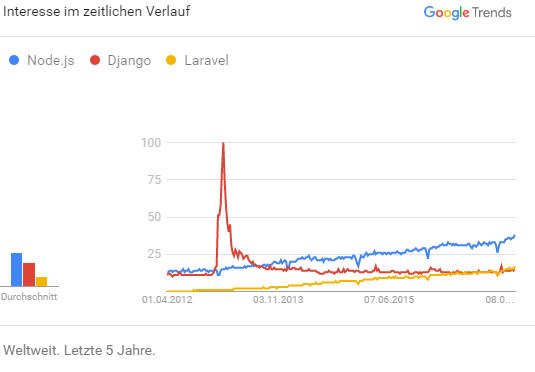
\includegraphics[width=3.8in]{images/framework_trends}
    \caption{Google Trends der evaluierten Frameworks\cite{frameworks_trends}}
\end{figure}

\newpage

%%%%%%%%%%%%%%%%%%%%%%%%%%%%%%%%%%%%%
%         Datenübermittlung         %
%%%%%%%%%%%%%%%%%%%%%%%%%%%%%%%%%%%%%
\subsection{Art der Daten\"ubermittlung}
Bei der Daten\"ubertragung sind mehrere Parameter zu beachten. Dazu geh\"oren haupt-s\"achlich das Format der Daten und das Intervall in denen diese \"ubertragen werden.
\subsubsection{Arduino zu Raspberry Pi und vice versa}
Um die Sensordaten dem Raspberry Pi mitzuteilen, eignet sich am besten ein Key-Value Format. Dabei gibt es verschiedene M\"oglichkeiten, wie z.B. \gls{JSON} und \gls{CSV}. \\
Das Intervall der Daten\"ubertragung kann frei, vom Benutzer gew\"ahlt werden.
\paragraph{\gls{JSON}} \mbox{}\\
\gls{JSON} (JavaScript Object Notation) hat den gro{\ss}en Vorteil, der leichten Server-seitigen Auswertung und Konvertierung in ein Javascript Objekt. Da die Daten aber \\ vorübergehend auf dem Raspberry Pi persistiert werden sollen, und Redis kein automatisches speichern von \gls{JSON} Objekten unterst\"utzt erzeugt diese Methode der \"Ubertragung mehr Aufwand als Nutzen.
\paragraph{\gls{CSV}} \mbox{}\\
\"Ahnlich wie bei \gls{JSON}, m\"ussten die Daten erst bearbeitet und gefiltert werden, um in die Datenbank gespeichert werden zu k\"onnen.
\paragraph{Eigenes Format} \mbox{}\\
Da die Daten in einer Redis Datenbank auf dem Key-Value Prinzip basieren, können die Daten auch entsprechend übertragen werden. Ein Key-Value-Paar wird in einer Zeile übertragen ("`ph 7.2\textbackslash n"')
\paragraph{Fazit} \mbox{}\\
Der Datenaustausch zwischen Arduino und Raspberry Pi wird in folgendem Format stattfinden:
\begin{lstlisting} [frame=single, caption=Datenaustauschformat zwischen Raspberry Pi und Arduino]
	tp 18.2
	ph 7.2
	ec 286.4
\end{lstlisting}

\newpage
\subsubsection{Raspberry Pi zu Server und vice versa}
Nachdem die Daten in Redis gespeichert wurden, werden diese zum Zentralserver gesendet. Node.js wird sowohl als Client als auch als Empfänger verwendet.

Die Daten sehen bei Auslesen der Datenbank wie folgt aus:
\begin{lstlisting} [frame=single, caption=Daten beim Auslesen der Datenbank]
	1) tp
	2) 23.4
	3) ec
	4) 285.7
\end{lstlisting}

Wie in Kapitel 4.6.1 festgestellt, offenbart sich die \"Ubertragung in \gls{JSON} nicht nur wegen der Einfachheit der Konvertierung zu einem Javascript Objekt als Vorteil, sondern auch aus drei anderen Gr\"unden:
\begin{itemize}
    \item \textbf{Einfache Speicherung in MongoDB:} Da MongoDB \gls{JSON} als Speicherformat verwendet, ist es deswegen f\"ur uns einfacher \gls{JSON}-Objekte in die Datenbank zu speichern.
    \item \textbf{\"Ubertragung der Daten durch Socket.io:} Daten werden standardm\"a{\ss}ig in Socket.io als \gls{JSON}-Objekt gesendet.
    \item \textbf{Oberfl\"ache der Webapp durch Angular:} Angular bietet Funktionen an, \gls{JSON}-Objekte in der Weboberfl\"ache anzeigen zu lassen. Falls sich das \gls{JSON}-Objekt ver\"andert, wird automatisch auch die Oberfl\"ache dementsprechend angepasst.
\end{itemize}

Deswegen werden die Daten wie folgt aussehen:
\begin{lstlisting} [frame=single, caption=Datenformat]
	{
	  tp: "23.4",
	  ec: "285.7"
	}
\end{lstlisting}
\newpage
\subsection{Komponenten- und Kostenaufstellung}
Die Gesamtkosten ergeben sich aus den Unterpunkten Technik, Zubehör und Webpräsenz:
\begin{table}[ht]
{\centering
\begin{tabular}{c|c}
Summe Technik    & 313,78 € \\
Summe Zubehör    & 186,78 € \\
Summe Webpräsenz & 50,00 €  \\ \hline
\textbf{Gesamtbetrag}     & \textbf{550,56 €}
\end{tabular}
\caption{Gesamtsumme der Kosten}}
\end{table}

\mbox{} \\
Die Kosten, um unsere Webpräsenz, sowie die Web-App, zu hosten, belaufen sich auf folgende Unterpunkte:
\mbox{} \\

\begin{table}[ht]
{\centering
\begin{tabular}{|c|c|}
\hline
\textbf{Artikel}       & \textbf{Einkaufspreis} \\ \hline
Server OVH-VPS         & 20,00 € per 6 Monate   \\ \hline
Domain (urbangreen.io) & 30,00 € pro Jahr       \\ \hline
\end{tabular}
\caption{Webpräsenz Kosten}}
\end{table} \mbox{} \\
In der unten stehenden Tabelle sind alle verbauten Komponenten, dessen Stückzahl und Einkaufspreis gelistet:\\

\begin{table}[ht]
\centering
\begin{tabular}{|c|c|c|}
\hline
\textbf{Artikel}                                                                                     & \textbf{Stückzahl} & \textbf{Gesamtpreis}   \\ \hline
\begin{tabular}[c]{@{}c@{}}Raspberry Pi Display\end{tabular}                                         & 1                  & 80,00 €                \\ \hline
\begin{tabular}[c]{@{}c@{}}Aquariumheizer, Eheim Thermocontrol\\ 200 Watt\end{tabular}               & 1                  & 22,99 €                \\ \hline
Luftpumpe, Eheim air pump 400                                                                        & 1                  & 27,99 €                \\ \hline
\begin{tabular}[c]{@{}c@{}}Außenpumpe, JBL Cristalprofi\\ E901\end{tabular}                          & 1                  & 89,00 €                \\ \hline
\gls{SBC}, Raspberry Pi 3B                                                                           & 1                  & 39,00 €                \\ \hline
Netzteil für Raspberry Pi 3B                                                                         & 1                  & 20,00 €                \\ \hline
RGB-LED Streifen                                                                                     & 1 (10 m)           & 25,00 €                \\ \hline
Jumperkabel                                                                                          & 1 (20 Stück)       & 5,00 €                 \\ \hline
Niedervoltbuchse                                                                                     & 1                  & 3,00 €                 \\ \hline
\gls{MOSFET}                                                                                         & 3                  & 1,80 €                 \\ \hline
\textbf{Gesamtsumme}                                                                                          & \textbf{-}                  & \textbf{313,78 €}               \\ \hline
\end{tabular}
\caption{Kostenaufstellung technische Einkäufe für den Prototypen}
\end{table}

\newpage
Um das Aquarium zu betreiben und Wartbarkeit beizubehalten, mussten diverse Artikel angeschafft werden. Diese Artikel umfassen diverse Wasseraufbereiter und Wasserpflegemittel, Aquariumkies und -sand aber ein Transportroller welcher ermöglicht das Aquarium, wenn benötigt (bei Wartarbeiten oder zum Beispiel Übersiedlung), erleichtert zu transportieren.\\
All diese gekauften Artikel werden in der folgenden Tabelle aufgelistet:
\begin{table}[ht]
\centering
\begin{tabular}{|c|c|c|}
\hline
\textbf{Artikel}                                                                     & \textbf{Stückzahl} & \textbf{Gesamtpreis}   \\ \hline
\begin{tabular}[c]{@{}c@{}}Aquarien Pflanzensand, \\ JBL Aquabasis plus\end{tabular} & 1 (5 l)            & 12,99 €                \\ \hline
Aquariumsand                                                                         & 2 * 4,5 l          & 8,98 €                 \\ \hline
Aquariumkies                                                                         & 2                  & 15,98 €                \\ \hline
\begin{tabular}[c]{@{}c@{}}Kunststoff Baumstamm\\ Fischversteck\end{tabular}         & 1                  & 17,99 €                \\ \hline
Keramik Fischversteck                                                                & 1                  & 16,99 €                \\ \hline
Deko Holzwurzelstamm                                                                 & 1                  & 12,99 €                \\ \hline
Deko Calari Stein                                                                    & 1                  & 5,95 €                 \\ \hline
Aquariumpflanzen                                                                     & 4                  & 11,16 €                \\ \hline
Aquariumschwamm JBL Spongi                                                           & 1                  & 1,95 €                 \\ \hline
AquaForte Eco-Check Teststreifen                                                     & 1 (50 Stück)       & 10,90 €                \\ \hline
Filtergel                                                                            & 1 (0,5 l)          & 12,50 €                \\ \hline
Aquariumreiniger, Sludge-Away                                                        & 1 (1 l)            & 16,50 €                \\ \hline
Eisendünger 6\%                                                                      & 1 (70 g)           & 5,00 €                 \\ \hline
\begin{tabular}[c]{@{}c@{}}Transportroller, \\Bauhaus Eigenmarke bis zu \\400 kg Traglast\end{tabular}                           & 1                  & 36,90 €                \\ \hline
\textbf{Gesamtsumme}                                                                          & \textbf{-}                  & \textbf{186,78 €}               \\ \hline
\end{tabular}
\caption{Aquarium Zubehör}
\end{table}

Die Entwicklung des System benötigt keine zusätzlichen Kosten, welche beispielsweise für Lizenzen benötigt werden.

\newpage
\subsection{Fazit des kompletten Systems}

Der Aufbau des kompletten System wurde in der folgenden Grafik veranschaulicht und basiert auf die Evaluierung.

\begin{figure}[ht]
    \centering
    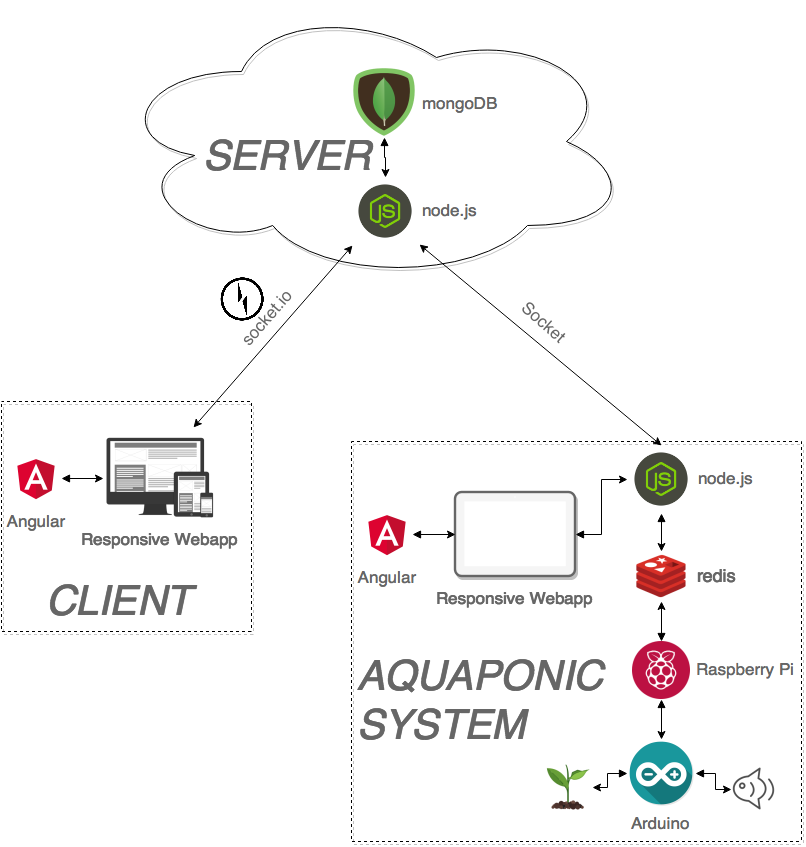
\includegraphics[height=5.5in]{images/complete_system}
    \caption{Aufbau komplettes System}
\end{figure}



\afterpage{\blankpage}

\subsection{Aufgabenstellung}
%\input{}

\subsection{Ziele und Zielgruppen}
%\input{}

\subsection{Konzept}
%\input{}

\newpage %----------------------------------------------------------------------------------------------

\section{Grundlagen und vorhandene Technologien}
%\input{}

\newpage %----------------------------------------------------------------------------------------------
\subsection{Methodiken zur Verbreitung}
%\input{}
\newpage

\subsubsection{Citizen Science}
%\input{}

\newpage
\subsubsection{Blidungssektor}
%\input{}

\subsection{Vorhandene Aquaponiksysteme}
%\input{}

\newpage
\subsubsection{Grove Ecosystem}
%\input{}

\subsubsection{EcoQube C}
%\input{}

\subsubsection{Ponix Systems}
%\input{}



\newpage %----------------------------------------------------------------------------------------------
\section{Projektmanagement}
%\input{}

\subsection{Projektmanagement Methode}
%\input{}

\subsection{Teamstruktur}
%\input{}

\subsection{Aufgabenteilung}
%\input{}

\subsection{Terminplanung}
%\input{}

\subsection{User Stories}
%\input{}

\subsection{Sprint Dokumentation}
%\input{}

\newpage %----------------------------------------------------------------------------------------------
\section{Evaluierung der benötigten Technologien und Komponenten}
\section{Evaluierung von Technologien und Komponenten}
\setcounter{page}{27}
Damit die Anforderungen an das Projekt (Kapitel 3.5) erfüllt werden konnten, mussten folgende Hardware und Technologien evaluiert werden:
\begin{itemize}
    \item Hardware als Schnittstelle zwischen Sensorik und Webapp
    \item Sensoren und Aktoren
    \item Datenbankmanagementsystem
    \item Webframework
\end{itemize}
Rahmenbedingungen für diese Technologien, sind die von Ponix Systems zur Verfügung gestellten Elemente, wie zum Beispiel das 150 Liter Aquarium und der dazugehörige \gls{NFT}-Kanal für die Pflanzen.

%%%%%%%%%%%%%%%%%%%%%%%%%%%%%%%%%%%%%
%                SBC                %
%%%%%%%%%%%%%%%%%%%%%%%%%%%%%%%%%%%%%
\subsection{Single Board Computer}
\cfoot{Matthias Schwebler}
Um die Sensoren und Aktoren anzusprechen wird ein \gls{SBC} (Single Board Computer) verwendet. Aufgrund der Anzahl an erh\"altlichen \gls{SBC}s, wird der Fokus auf popul\"are Produkte mit  gro{\ss}er Community gelegt. Ideal w\"are ein \gls{SBC}, der auf Messger\"ate, wie sie im Aquarium verwendet werden, spezialisiert ist und ein \gls{WLAN}-Interface, f\"ur die Daten\"ubermitlung hat. Des Weiteren sollte er einen internen Speicher bieten (zusätzlich zum Betriebssystem für den Redis-Server (812 kB)\cite{redis_server_xenial} + Sensordaten) um im Falle eines Netzwerkausfalles, f\"ur einige Stunden alle Daten zwischenspeichern zu k\"onnen. 

\subsubsection{Modelle}
\myparagraph{Arduino}
Der Arduino Uno ist ein \gls{SBC}, welcher im Bereich von \euro20 - \euro25 zu erhalten ist \cite{AmazonArduino}. Er hat einen internen Speicher der gro{\ss} genug ist, um einen Netzwerkausfall \"uberbr\"ucken zu k\"onnen. Da er aber selbst keine Netzwerkschnittstelle hat, muss er mit einem WiFi-Shield (\euro 90) ausgestattet werden. Ein Shield ist eine Hardware-Erweiterung, die dem Arduino situationsbezogene Funktionen hinzuf\"ugen kann. F\"ur dieses Projekt ist das "`Open Aquarium Board"' (\euro 60) \cite{OpenAquariumBoard} optimal, da es speziell für die \"Uberwachung bzw. Steuerung entwickelt wurde. Es bietet außerdem eine Open Source \gls{API} an. \\ \mbox{} \\
Das Problem dabei ist, dass nur ein Shield auf dem Arduino angebracht werden kann. Das hei{\ss}t, entweder das Open Aquarium Board wird verwendet, oder ein Wifi-Shield zur Daten\"ubermittlung. Er m\"usste mit einem anderen \gls{SBC}, welcher netzwerktauglich ist, verbunden werden um die Daten auf einem zentralen Server zu persisiteren. \cite{ArduinoBoardUno}
\newpage
\myparagraph{Raspberry Pi 3 Model B}
Der Raspberry 3 (Model B) ist der derzeit aktuelle Raspberry Pi (Stand: November 2016). Wie bei den anderen Raspberry Pi's hängt der Speicherplatz von der verbauten SD Karte ab. Dieser Raspberry Pi unterscheidet sich von den anderen, mit seinem eingebauten \gls{WLAN}-Chip, was den Vorteil bringt, dass kein zusätzlicher \gls{USB}-Stick verwendet werden muss. Der Raspberry Pi kann genug Strom aufnehmen um Peripheriegeräte anzuschließen. Allerdings ist ein großer Nachteil, gegenüber dem Arduino, dass keine API zur Verfügung steht um etwaige Sensoren und Aktoren anzusprechen. Es erfordert also einen höheren Programmieraufwand die Sensoren über den Raspberry Pi zu betreiben als über einen Arduino. 
\myparagraph{Raspberry Pi Zero}
Ebenso wie andere Raspberry Pi's, hat der Pi Zero einen erweiterbaren Speicher und kann mit einem \gls{WLAN}-Stick mit einem Lokalen Netzwerk verbunden werden. Der Unterschied ist, dass er keine \gls{RJ45} Buchse besitzt und um einiges weniger Rechnleistung bietet. Der Vorteil dabei ist, dass er sehr wenig Strom verbraucht (65mA im Leerlauf \cite{PiPower}).\cite{PiZero}
\myparagraph{L\"osung}
Aus Erfahrungswerten der Firma Ponix Systems, ist das Open Aquarium Board f\"ur den Arduino unabdinglich. Die optimale L\"osung ist also, ein Arduino mit entsprechendem Shield, der die Daten an einen Raspberry Pi \"ubermittel, welcher diese dann an einen Server schickt. Da der Raspberry in der Lage sein muss die Webapp einwandfrei zu betreiben, wurde auf den Raspberry 3 Model B gesetzt, da dieser die notwendige Leistung erbringen kann. 

\newpage
\subsubsection{Software}
\myparagraph{Image für die Auslieferung}
Das \gls{OS} eines Raspberry Pi's befindet sich auf der Speicherkarte. Um später nicht jedes Gerät einzeln konfigurieren zu müssen, wird ein Image erstellt, auf dem alle benötigten Programme und Dateien enthalten sind. Als Basis dient die Standardoberfläche "`Raspbian"' (Raspbian Jessie with matchbox-window-manager). Da diese nicht alle notwendigen Programme beinhaltet, werden diese nachträglich installiert. \\ 
Zusätzlich installierte Softwarepakete:
\begin{itemize}
    \item npm
    \item nodeJs
    \item python-pip
\end{itemize}
Benötigte Python libraries:
\begin{itemize}
    \item redis
    \item serial
    \item time
    \item os
    \item re
    \item thread
    \item RPi (GPIO)
    \item datetime
    \item sys
\end{itemize}
\newpage

%%%%%%%%%%%%%%%%%%%%%%%%%%%%%%%%%%%%%
%              Aktoren              %
%%%%%%%%%%%%%%%%%%%%%%%%%%%%%%%%%%%%%
\subsection{Aktoren}
Es wurden insgesamt vier Aktoren von Ponix Systems zur Verf\"ugung gestellt:
\begin{itemize}
    \item Wasserpumpe
    \item Mineralienpumpe
    \item Futterautomat
    \item Pflanzenbeleuchtung
\end{itemize} 
Zusätzlich wird ein RGB-LED-Streifen verbaut.
Da die Fische auch im Bezug auf die Temperatur äußerst empfindlich sind wird zusätzlich ein Hitzestrahler verbaut. Dadurch wird die Benutzerfreundlichkeit weiter verbessert. Alle dafür nötigen Arbeitsschritte werden im Kapitel 4.3.5 genauer erläutert. \\ \mbox{} \\
Alle folgenden Abbildungen, die die Anschlussmöglichkeiten der Sensoren und Aktoren beschreiben, wurden von cooking-hacks übernommen. \cite{OpenAquarium}
\subsubsection{Wasserpumpe}
Eine Wasserpumpe muss verwendet werden, um das Wasser des Aquariums durch den \gls{NFT}-Kanal zu pumpen, welcher die Pflanzen mit den notwendigen Nährstoffen versorgt. 
\myparagraph{Option 1: Cooking Hacks}
Die Wasserpumpe von cooking-hacks.com kann mit einer Zeile Code ein bzw. ausgeschalten werden.

\begin{lstlisting} [frame=single, caption=Steuern der Wasserpumpe von cooking-hacks]
OpenAquarium.pumpON(1); // switch pump nr 1 on
OpenAquarium.pumpOFF(1); // switch pump nr 1 off
\end{lstlisting}
\newpage
Zum Anschlie{\ss}en der Pumpe sind auf dem AquariumBoard Steckplätze vorgesehen. \\
\begin{figure}[ht]
    \centering
    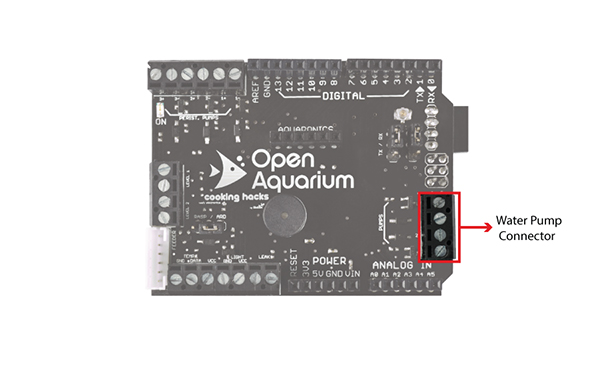
\includegraphics[height=2in]{images/water_pump_connection}
    \caption{Anschluss der Wasserpumpe}
\end{figure} \\
Pumpleistung: 100-350 l/h \\
Spannung: 3.5-12V DC \\
Leistungsbereich: 0.5W-5W \cite{WaterPump}\\
\myparagraph{Option 2: Handelsübliche Aquariumpumpe}
Die Pumpe von cooking-hacks.com ist sehr klein und würde gerade einmal reichen um die Pflanzen mit Wasser zu versorgen. Um aber den Wasserkreislauf des Aquariums (150 Liter) zu regeln, ist sie um einiges zu schwach. \\ \mbox{} \\
Es müsste also eine zusätzliche Pumpe eingebaut werden um diesen Kreislauf zu regulieren. Dadurch wird die Pumpe von cooking-hacks.com redundant, weil sie einfach durch eine Erweiterung des Wasserkreislaufes ersetzt werden kann, sodass das Blumenbeet über einen \gls{NFT}-Kanal mit einbezogen ist. Das Wasser wird also vom Aquarium durch den Filter der Außenpumpe geleitet um anschließend die Pflanzen über den \gls{NFT}-Kanal zu düngen und wieder zurück ins Aquarium zu fließen.\\ \mbox{} \\
Es wurde also einzig und allein auf eine normale (statische) Außenpumpe (JBL Cristalprofi E901 Greenline) gesetzt. Diese ist mit einer Pupmleistung von 900 l/h für das verwendete 120x40x50cm große Aquarium bestens geeignet. \cite{JBL}

\newpage
\subsubsection{Mineralienpumpe}
Bei dieser Pumpe handelt es sich um eine Schlauchpumpe. Eine Schlauchpumpe treibt ein Medium durch, von außen einwirkende Rollen, durch einen Schlauch. Sie ist auf einzelne Tropfen genau und eignet sich deshalb gut um  empfindliche Parameter eines Ökosystems mithilfe von speziellen Lösungen zu regulieren. Es können insgesamt drei Pumpen angeschlossen werden, wobei im Normalfall werden zwei davon an Gefäße mit Flüssigkeiten mit einem pH-Wert von 4 und 10 angehängt werden. \cite{hitec-zang} \\ \mbox{} \\
Wie bei der Wasserpumpe ist der Code zum Aktivieren und Deaktivieren der Pumpe kurz.
\begin{lstlisting} [frame=single, caption=Steuern der Peristaltikpumpe]
OpenAquarium.perpumpON(1); // switch pump nr 1 on
OpenAquarium.perpumpOFF(1); // switch pump nr1 off
\end{lstlisting}
Zum Anschließen der Pumpen sind ebenfalls Steckplätze vorhanden. \\
\begin{figure}[ht]
    \centering
    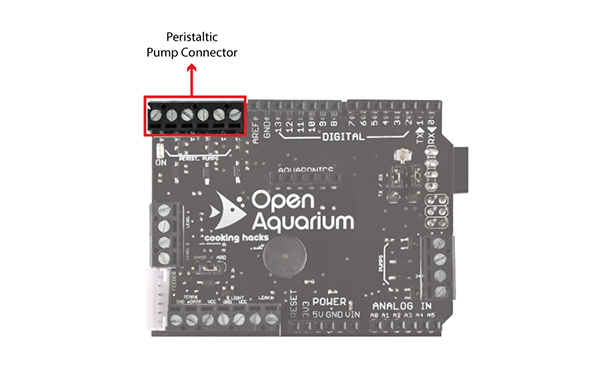
\includegraphics[height=2.1in]{images/mineral_pump_connection}
    \caption{Anschluss der Peristaltikpumpe}
\end{figure} \\
12V DC input voltage \\
Flow: 20-60 ml/min \cite{PeristaltikPump}
\newpage
\myparagraph{Fazit}
Die automatische Regulierung des pH-Wertes sollte nicht auf Dauer (mehr als 2 Monate) verwendet werden, da der pH-Wert Sensor mit der Zeit verschleißt und verfälschte Ergebnisse liefert. Abgesehen davon ist die Regulierung des pH-Wertes auch nur zu Beginn bzw. nach der Besetzung eines Aquaponik-Systems essentiell, da gerade in dieser Zeitspanne der pH-Wert instabil ist.  \\ \mbox{} \\
Da während dem Projekt aus finanziellen Gründen lediglich eine einzige Schlauchpumpe - anstatt der vorgesehenen \textit{drei} - zur Verfügung stand, wurde diese nicht zum Regulieren des pH-Wertes, sondern zum Einspeisen von spezialisierten Minerallösungen in das Aquarium verwendet. \\ \mbox{} \\
Auf Seiten der Software, wären alle Möglichkeiten gegeben, alle drei Pumpen zu implementieren, jedoch konnte aufgrund der Kosten der Pumpen im Rahmen dieses Projektes nur eine der beschriebenen Möglichkeiten umgesetzt werden. 

\newpage
\subsubsection{Futterautomat}
Um den Wartungsaufwand zu minimieren, war ein Futterautomat notwendig, der \"uber eine Weboberfl\"ache konfiguriert werden kann. Es konnte entweder auf einen teuren Futterautomaten gesetzt werden, der diese Option anbietet, oder ein handelsüblicher Futterautomat wird so bearbeitet, dass er als Reaktion auf ein Stromsignal Futter ausgibt. \\
Der Futterautomat von Ponix Systems geh\"ort zur letzteren Art. Sobald 5 Volt angelegt wird, gibt er Futter aus. So kann \"uber die Webapp das Intervall und die Menge gesteuert werden. \\
Da die \gls{GPIO} Pins des Raspberry Pi's allerdings nur 3,3 Volt liefern, musste entweder ein Spannungsteiler verwendet werden, oder ein Transistor, der an 5 Volt angelegt ist und entsprechend durchgeschaltet wird. Da der 5 Volt Ausgang ohnehin nicht gebraucht wird, wird auf die Lösung mit dem Transistor zurückgegriffen. Dafür wird ein "`General Purpos Transistor"' mit einem PNP-Übergang verwendet, welcher in einem Bereich von 0 bis maximal 50 Volt arbeitet und somit für den vorgesehenen Verwendungszweck geeignet ist. \cite{BC557} \\ \mbox{} \\
Die Bezeichnung des Transistors lautet: \texttt{BC557}
\\ \mbox{} \\
Das folgende Script soll beispielhaft zeigen wie der Futterautomat, der nach dem eben beschriebenen Aufbau angeschlossen ist, anzusteuern ist.
\begin{lstlisting}[language=Python]
import RPi.GPIO as GPIO
import time

GPIO.setmode(BOARD)
GPIO.setup(10, GPIO.OUT)

GPIO.output(10, GPIO.HIGH)
time.sleep(5)   # activate for 5 seconds
GPIO.output(10, GPIO.LOW)

GPIO.cleanup()
\end{lstlisting}
\newpage
Der Schaltplan für den beispielhaften Code sieht demnach wie folgt aus: \\ \mbox{} \\
\begin{figure}[ht]
    \centering
    \includegraphics[width=12cm]{images/fishFeeder}
    \caption{Schaltplan für den Futterautomaten}
\end{figure}
\newpage
\subsubsection{Pflanzenbeleuchtung}
\myparagraph{Option 1: Cooking Hacks}
Die Beleuchtung könnte mit einem \gls{LED} Streifen (www.cooking-hacks.com) realisiert werden. Er besteht aus 72 LEDs (60 Weiße und 12 Blaue) mit einer Leuchtkraft von 500 Lumen. Der Streifen kann mit Hilfe der OpenAquarium Klasse der aktuellen Zeit automatisch angepasst werden. Der folgende Code, steuert die Lampe so, dass sie für die Pflanze eine Sonne simuliert.
\begin{lstlisting} [language=C, caption=Steuerung des LED-Streifens von cooking-hacks]
now = OpenAquarium.getTime();
OpenAquarium.printTime(now);
OpenAquarium.lighting(now);
\end{lstlisting}
Wie bei den beiden Pumpen kann der \gls{LED} Streifen am OpenAquarium Board angeschlossen werden. \\
\begin{figure}[ht]
  \centering
    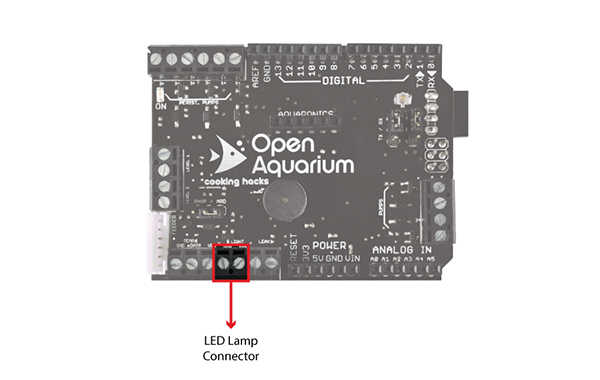
\includegraphics[height=1.8in]{images/led_connection}
    \caption{Anschluss der Beleuchtung}
\end{figure} \\
Leistung: 5.5 watts \\
Beleuchtung: 72 \gls{LED}s \\
Farbe: 60 Weiße + 12 Blaue \cite{LEDLamp}\\

\newpage
\myparagraph{Option 2: Eigenbau von Ponix Systems}
Als Alternative wird ein LED-Brett von Ponix Systems zur Verfügung gestellt. Dieser hat die Fähigkeit einige, für Pflanzen, wichtige Lichtspektren auszustrahlen. Es benötigt eine Stromversorgung mit 24 Volt und ein pulsierendes Signal auf dem EN-Eingang. Dieses Signal wird verwendet um die Intensität des Lichtes zu steuern, indem eine gewisse Frequenz vom Raspberry Pi gesendet wird. Dazu wird ein so genannter \gls{PWM}-Pin (Pulsweitenmodulation) verwendet. Aus Erfahrungswerten der Firma Ponix Systems, ist diese Lösung deutlich besser für die Wachstumsdauer der Pflanzen. \cite{osram, elektrJournal} \\ \mbox{} \\
Die LED-Bretter haben jeweils drei Eingänge: +, -, EN \\
Es wird also auf die Lösung von Ponix Systems zurückgegriffen, welche einen höheren Programmieraufwand erfordert, dafür allerdings einen großen Vorteil für die Pflanzen. Die Qualität könnte immer noch durch besser spezialisierte Beleuchtung weiter verbessert werden (Siehe 8.1.3). 
\begin{figure}[ht]
    \centering
    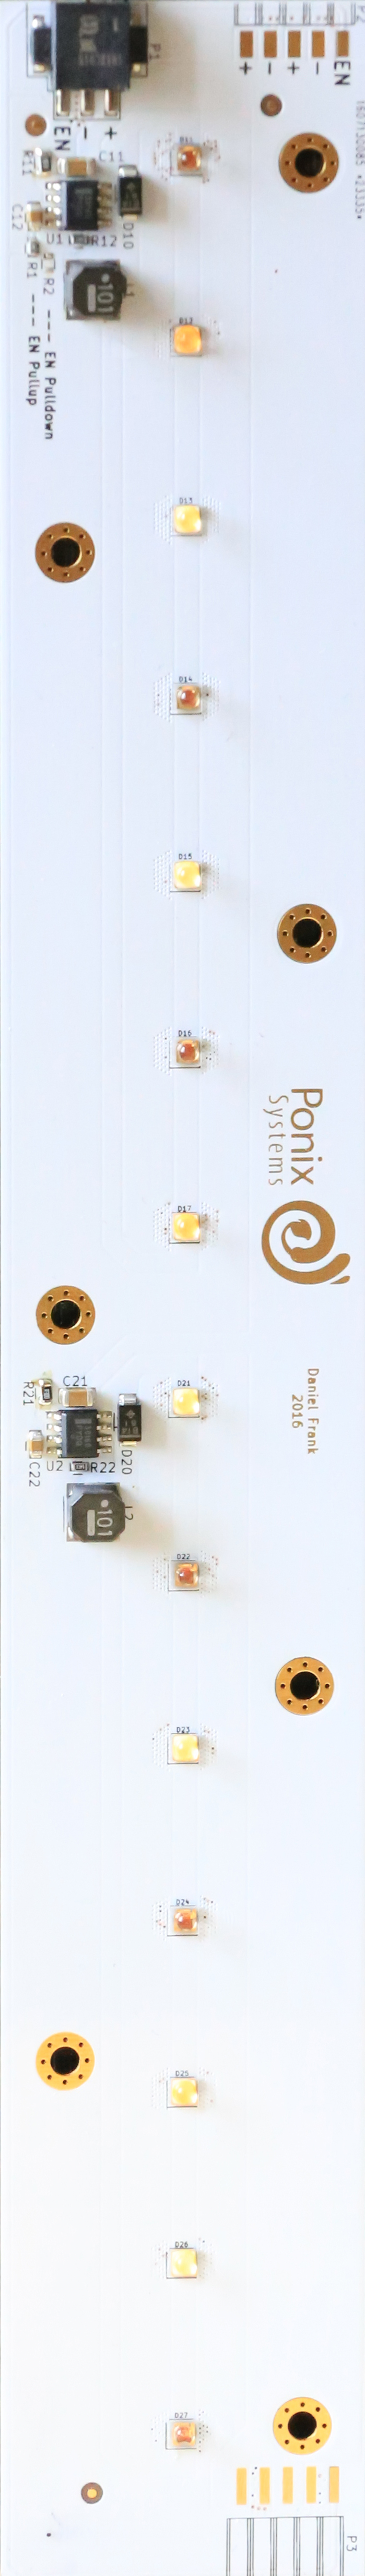
\includegraphics[angle=90, width=15cm]{images/pflanzenLicht}
    \caption{Lichtstreifen von Ponix Systems}
\end{figure} \\ \mbox{} \\
Der Aufbau der Schaltung sieht demnach wie folgt aus: \\
\begin{figure}[ht]
    \centering
    \includegraphics[height=8cm]{images/LED-Brett-Anschluss}
    \caption{Schaltung für LED-Bretter}
\end{figure} 
\newpage
Wenn die Pflanzenbeleuchtung nach der eben gezeigten Schaltung aufgebaut ist, kann die Intensität mithilfe der Frequenzregulierung des PWM-Pins gesteuert werden. Im folgenden Beispielcode wird das LED-Brett für eine Stunde mit einer Intensität von 50 Prozent aktiviert.
\begin{lstlisting}[language=Python, caption=Steuern der Pflanzenbeleuchtung]
import RPi.GPIO as GPIO
import time

GPIO.setmode(GPIO.BOARD)
GPIO.setup(12, GPIO.OUT)
light = GPIO.PWM(12, 100)
light.start(50)  # start with intensity of 50 percent
time.sleep(3600) # expose for 1 hour
light.ChangeDutyCycle(0) # set intensity to 0

GPIO.cleanup()
\end{lstlisting}

\newpage
\subsubsection{Hitzestrahler}
Es gibt für das OpenAquarium Board keinen Hitzestrahler der entsprechend konfiguriert werden und eine bestimmte Temperatur halten kann. \\ \mbox{} \\
\begin{figure}[ht]
  \centering
  \includegraphics[height=2.2in]{images/heaterPipePlan}
  \caption{Schaltplan zum Steuern des Hitzestrahlers}
\end{figure} \mbox{} \\ \mbox{} \\
Am benutzerfreundlichsten erschien es den Hitzestrahler auf die höchstmögliche Temperatur einzustellen und je nach aktueller Temperatur, und der vom Benutzer über die Webapp angegebenen Wunschtemperatur, des Aquariums, das Relais zu aktivieren bzw. zu deaktivieren. \\ \mbox{} \\
Das Problem beim Steuern des Hitzestrahlers über das Internet ist, dass einige Störfak-toren einwirken. Daten könnten geändert/gefälscht werden, der Sensor könnte falsche Daten liefern, das Relais könnte eine Fehlfunktion aufweisen. Wenn eine dieser Fälle eintritt, wird das Aquarium so warm, dass sämtliche Fische sterben würden. Daher ist es sinnvoller den Hitzestrahler nicht über das Netzwerk zu steuern, sondern manuell einzurichten. Der Benutzer muss also lokal, den Hitzestrahler an seine Bedürfnisse anpassen. 
\newpage
%%%%%%%%%%%%%%%%%%%%%%%%%%%%%%%%%%%%
%               LED                %
%%%%%%%%%%%%%%%%%%%%%%%%%%%%%%%%%%%%
\subsubsection{RGB-LED-Streifen}
Um das Aquarium von innen heraus zu beleuchten, werden wasserdichte \gls{RGB}-\gls{LED}-Streifen verbaut. Dabei soll die Intensität der einzelnen Farben (Rot, Grün und Blau) über die Webapp angepasst werden können, um so die gesamte Farbe zu regulieren. Um dies zu ermöglichen, wurden die einzelnen Kanäle über eine Schaltung mit dem Raspberry Pi verbunden. Diese Schaltung besteht aus drei MOSFET's, die jeweils einen Farbkanal übernehmen, wie in der Graphik auf der folgenden Seite zu sehen ist (Abbildung 12). \\ \mbox{} \\
Um eine bestimmte Farbe zu aktivieren, wird das Programm und Python Library \texttt{pigpio} verwendet. Mit der Kommandozeile kann beispielsweise die Farbe "`Karminrot"' - rgb(161, 35, 43) - mit folgendem Befehl eingerichtet werden:
\begin{center}
    \texttt{sudo pigpiod pigs p 40 161 pigs p 38 35 pigs p 38 43}
\end{center} \mbox{} \\
Konkret wird mit diesem Kommando gleichzeitig der \texttt{pigpiod}-Daemon gestartet und Parameter für die Steuerung der Pins übergeben. Der Daemon kann zur Laufzeit GPIO-Pins steuern, indem Nachrichten an ihn gesendet werden. Diesen Teil übernimmt \texttt{pigs}. Mit \texttt{pigs} wird die Pulsweitenmodulation eines GPIO-Pins angepasst und aktualisiert. Mit Hilfe dieser Frequenz und der verbauten Schaltung (Abbildung 9) können die einzelnen Farben (Rot, Grün und Blau) einzeln gesteuert werden.
\begin{figure}[ht]
    \centering
    \includegraphics[width=7cm]{images/pigs.png}
    \caption{Syntax von pigs}
\end{figure}
\begin{figure}[hp]
    \centering
    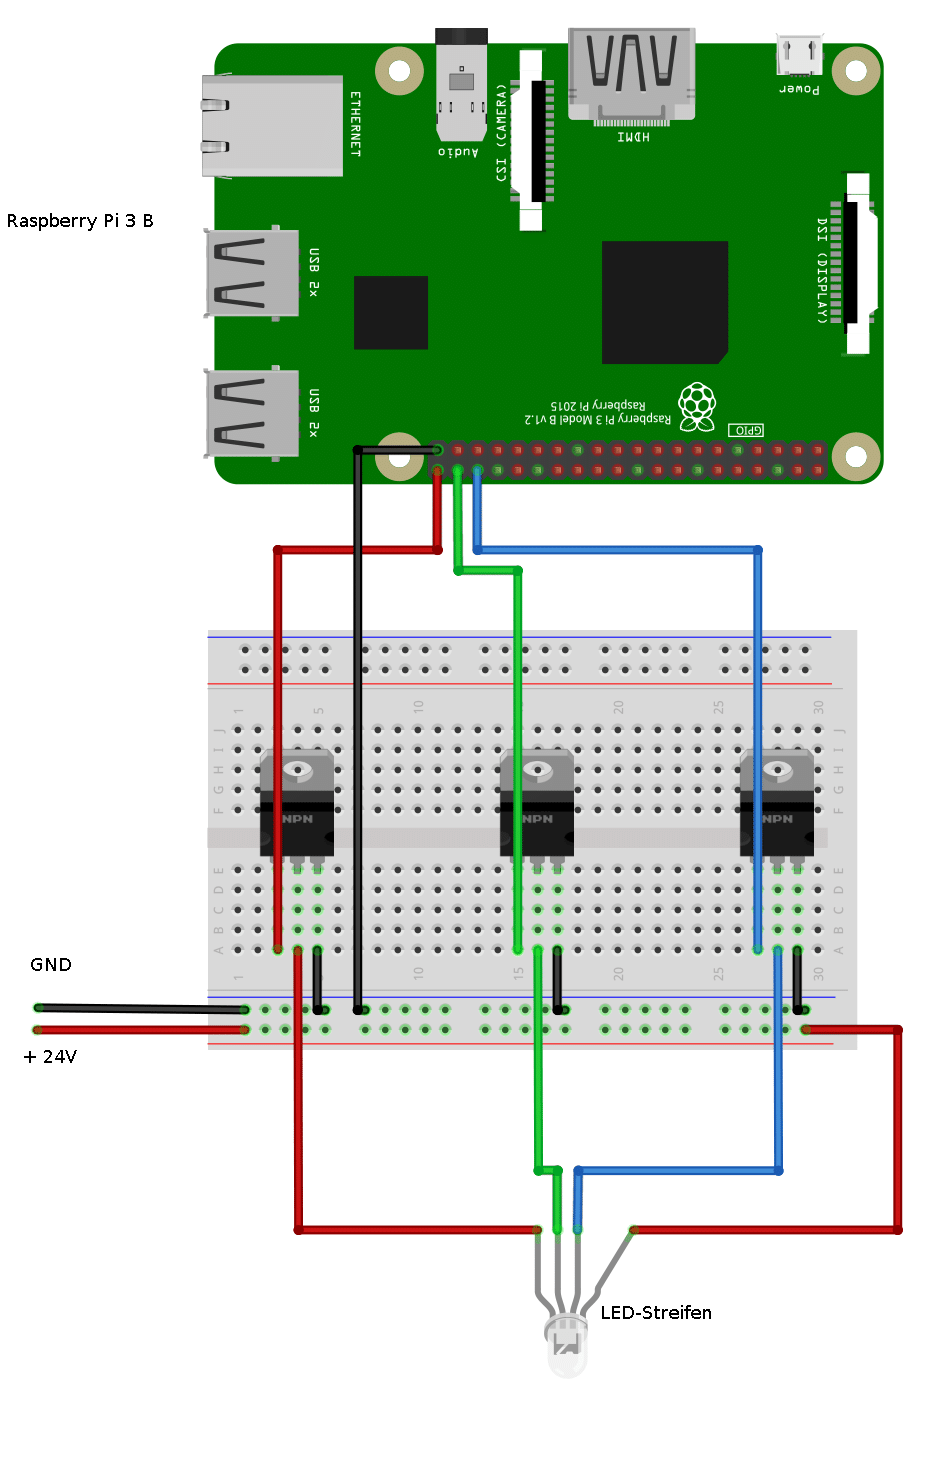
\includegraphics[width=13cm]{images/led_stripe}
    \caption{RGB-LED-Streifen Schaltplan}
\end{figure}

\newpage
%%%%%%%%%%%%%%%%%%%%%%%%%%%%%%%%%%%%%
%             Sensoren              %
%%%%%%%%%%%%%%%%%%%%%%%%%%%%%%%%%%%%%
\subsection{Sensoren}
Die Sensoren f\"ur den Prototypen, werden von der Firma Ponix Systems zur Verf\"ugung gestellt. Diese mussten allerdings erst auf Funktionalit\"at untersucht werden. \\
F\"ur die Entwicklung, des Codes, zum Ansprechen der Sensoren, wird "`Arduino \gls{IDE}"' verwendet. Diese \gls{IDE} bietet die M\"oglichkeit, den Code auf einem rechenstarken PC zu kompilieren und ihn dann auf dem Arduino auszuf\"uhren. Zus\"atzlich kann sie verwendet werden, um alle eingehenden Daten des Arduinos zu \"uberwachen.
Der kompilierte Code wird beim Endprodukt auf dem Arduino gespeichert und sendet kontinuierlich Daten \"uber die \gls{USB} Schnittstelle an den Raspberry Pi. Es werden Libraries von Arduino indirekt \"uber die \gls{API} von OpenAquarium verwendet. \\ \mbox{} \\
Alle folgenden Abbildungen, die die Anschlussmöglichkeiten der Sensoren und Aktoren beschreiben,wurden von cooking-hacks übernommen. \cite{OpenAquarium}

\newpage
\subsubsection{Temperatur}
Zum Messen der Temperatur wird der Sensor von www.cooking-hacks.com verwendet (DS18B20): \\
Input: 3.0-5.5V  \\
Arbeitsbereich: -55\degree C bis +125\degree C  \\
Genauigkeit: $\pm$ 0.5\degree C von -10\degree C bis +85\degree C \cite{TempSensor} \\
\mbox{}\\
Die Temperatur kann mit nur einem Befehl abgelesen werden. Dieser liefert einen Wert in Grad Celsius zur\"uck.
\begin{lstlisting} [language=C, caption=Auslesen der Temperatur]
OpenAquarium.init();
float temperature = OpenAquarium.readtemperature();
\end{lstlisting}
Die Testergebnisse des Temperatur Sensors stimmten mit den Werten eines handelsüblichen Thermometers überein.  \mbox{} \\
Angeschlossen werden die Sensoren bzw. der Temperatursensor auf dem OpenAquarium Board: \\
\begin{figure}[ht]
	\captionsetup{justification=raggedright}  
	\begin{minipage}[b]{.4\textwidth}  
		\centering  
		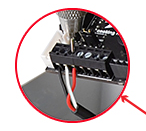
\includegraphics[width=3.5cm]{images/temp_sensor_connection_detail}  
	\end{minipage}%  
	\begin{minipage}[b]{0.6\textwidth}  
		\centering  
		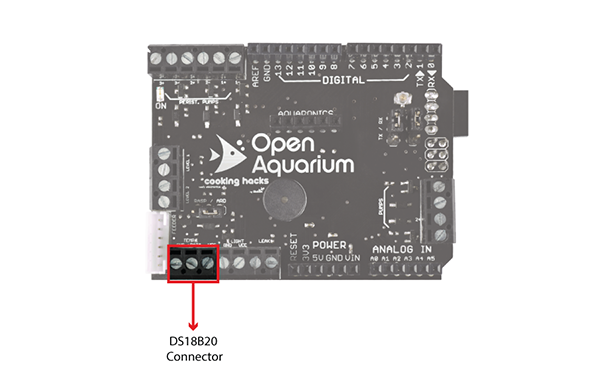
\includegraphics[width=8cm]{images/temp_sensor_connection}  
	\end{minipage}
	\par
	\begin{minipage}[t]{.4\textwidth}
		\centering  
		\caption{Detaillierte Darstellung der Anordnung der Kabel vom Temperatursensor}  
	\end{minipage}%
	\begin{minipage}[t]{.6\textwidth}  
		\centering  
		\caption{Anschluss des Temperatursensors}  
	\end{minipage}  
\end{figure}

\newpage
\subsubsection{EC Wert}
Der \gls{EC} Wert (Electrical Conductivity) gibt über die Leitfähigkeit des Wassers Auskunft. Mit diesem Wert kann grob auf die Menge der im Wasser gelösten Minerale/Salze geschlossen werden. Desto mehr N\"ahrstoffe im Wasser vorhanden sind, desto h\"oher ist auch der \gls{EC} Wert. \\ \mbox{} \\
Angeschlossen wird der Sensor auf dem OpenAquarium Board: \\
\begin{figure}[ht]
    \centering
    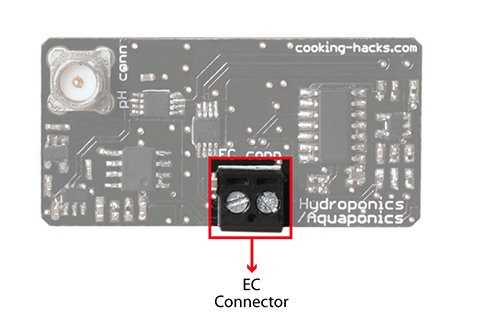
\includegraphics[height=2.0in]{images/ec_sensor_connection}
    \caption{Anschluss des \gls{EC}-Sensors}
\end{figure}

Um den EC Wert zu messen wird der Sensor von www.cooking-hacks.com verwendet, welcher mit folgendem Code angesprochen werden kann: \cite{TempSensor}

\begin{lstlisting} [frame=single, caption=Auslesen des EC Wertes]
OpenAquarium.init();
OpenAquarium.calibrateEC(point_1_cond,point_1_cal,
                         point_2_cond,point_2_cal);

float resistanceEC = OpenAquarium.readResistanceEC();
float EC = OpenAquarium.ECConversion(resistanceEC); //EC Value in uS/cm
\end{lstlisting}
\newpage
Die Tests beim Eintauchen des Sensors in Leitungswasser ergaben folgende Ergebnisse: \\
\begin{figure}[ht]
    \centering
    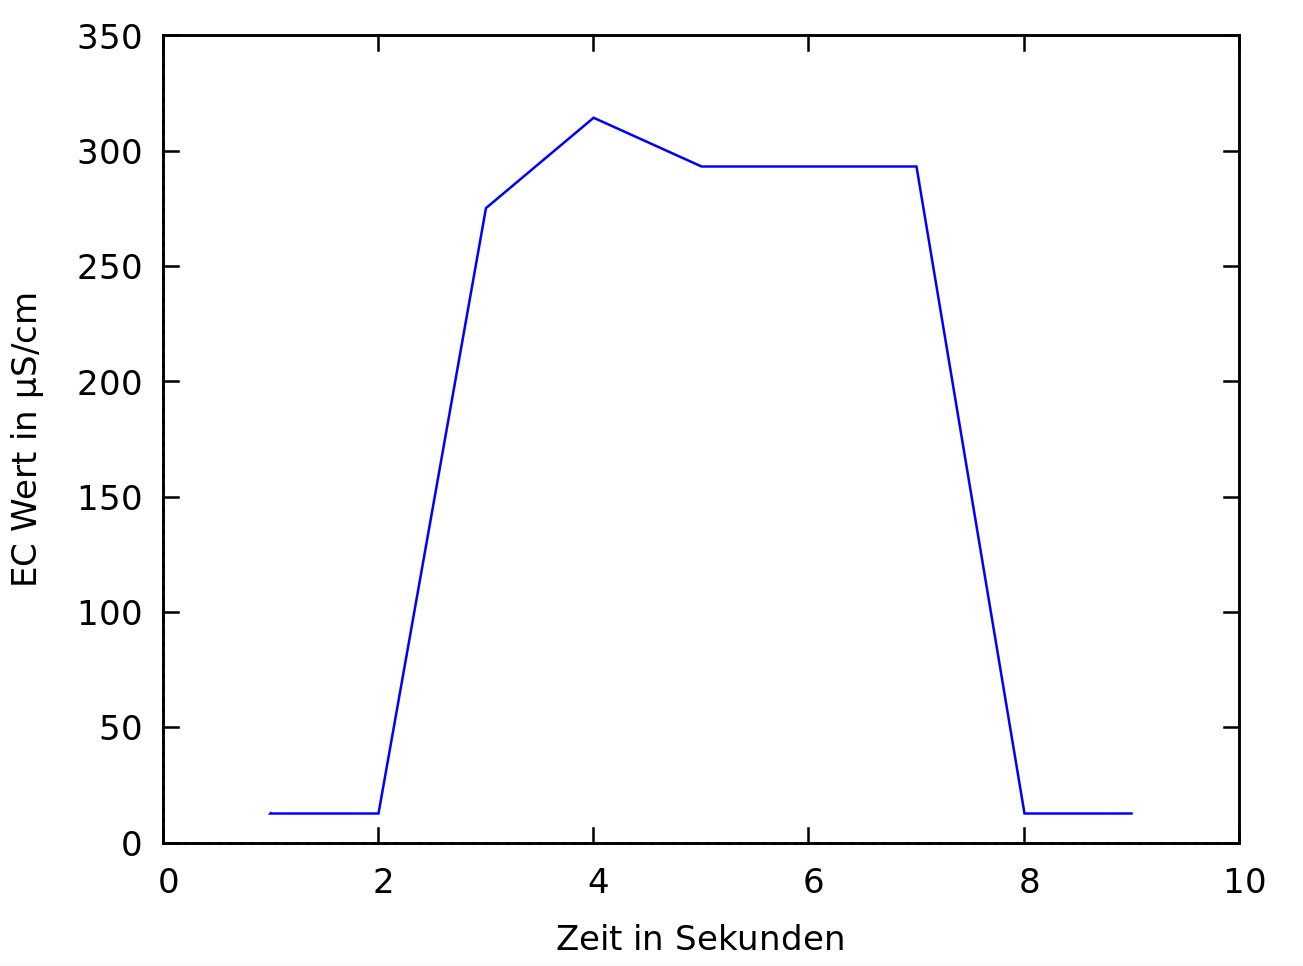
\includegraphics[height=3.2in]{images/ec_tests}
    \caption{Testergebnisse des EC-Sensors}
\end{figure}

\vskip0.5cm \mbox{} \\
Wie erwartet, steigt der \gls{EC} Wert beim Eintauchen ins Wasser, da es nat\"urlich um einiges leitf\"ahiger ist, als Luft. \\ \mbox{} \\

\newpage

\subsubsection{pH Wert}
Der pH-Wert ist einer der wichtigsten Werte, wenn es um das \"Uberwachen eines Aquaponik Systems geht. Es gibt ein gro{\ss}es Spektrum an erh\"altlichen Sensoren. Die der unteren Preisklasse, ben\"otigen regelm\"a{\ss}ige Wartungen, während die der oberen Preisklasse den Preis des Produktes, \"uber die Zielgruppe hinaus heben und somit unbrauchbar sind. Weil der Preis einer der ausschlaggebensten Punkte vom Homeponics System ist, musste auf einen billigen Sensor von www.cooking-hacks.com zurückgegriffen werden. Da allerdings die Überwachung des pH-Wertes gerade beim Besetzen eines Aquaponik Systems essentiell ist und danach nur noch gelegentlich geprüft werden muss, ist die Wartung nur zu Beginn von großer Bedeutung. Danach können je nach Stabilität des Ökosystems Wartungen ausgelassen werden. Da der Sensor ein analoges Signal liefert, muss die gemessene Spannung erst umgerechnet werden. Diese Aufgabe \"ubernimmt die Klasse OpenAquarium der OpenAquarium-Library für den Arduino (Siehe 4.2). \cite{pHsensor, abcChemie} \\

\begin{lstlisting} [frame=single, caption=Auslesen des pH-Wertes]
OpenAquarium.calibratepH(cp4,cp7,cp10);
int mvpH = OpenAquarium.readpH(); //Value in mV of pH
float pH = OpenAquarium.pHConversion(mvpH);
\end{lstlisting}
cp4, cp7, cp7 ... Calibrationpoints (Konstanten)

\paragraph{Calibrationpoints} \mbox{} \\
Zu den Calibrationpoints (Kalibrierungswerte) ist zu erwähnen, dass sie angepasst werden, wenn der gemessene pH-Wert zu stark vom eigentlichen Wert abweicht. Um die Abweichung des Sensors zu beheben, sind Kalibrierungskits vorgesehen, die allerdings bis zu ein mal im Monat verwendet werden m\"ussen. \\ \mbox{} \\
\newpage 
Angeschlossen wird der Sensor auf dem OpenAquarium Board. \\
\begin{figure}[ht]
    \centering
    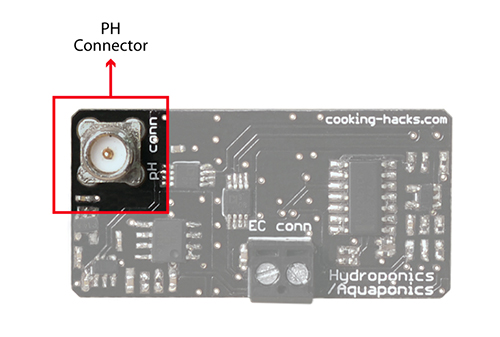
\includegraphics[height=2.0in]{images/ph_sensor_connection}
    \caption{Anschluss des pH-Sensors}
\end{figure}

\paragraph{Tests} \mbox{} \\
Beim Testen eines bereits l\"anger in Betrieb (2 Monate) gewesenem pH-Sensor brachte dieser folgende Ergebnisse: \\
\begin{figure}[ht]
    \centering
    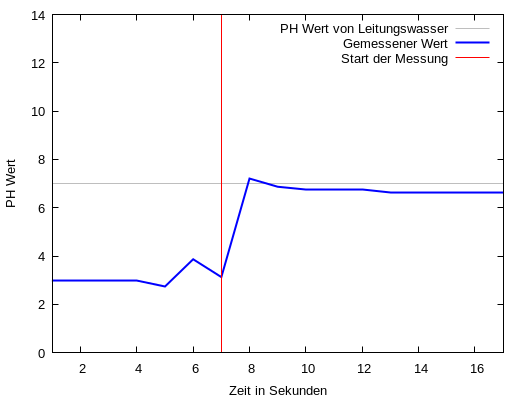
\includegraphics[height=2.7in]{images/ph_tests}
    \caption{Testergebnisse des pH-Sensors}
\end{figure} \\
Wie zu sehen ist, weicht der gemessene Wert bereits stark (0.5) von dem eigentlichen Wert ab. Für empfindliche Fische ist eine pH-Wertabweichung in diesem Ausmaß bereits tödlich. Ein Beispiel dafür, ist der Blaue Neon, dessen Lebensbereich zwischen einem pH-Wert von 5,5 und 6 eingegränzt ist, während die Guppies für ihre Robustheit von 6 - 8,5 beliebt sind. 
\paragraph{Fazit} \mbox{} \\
Da es keine pH-Sensoren gibt, die billig sind und zugleich einen niedrigen Wartungsauf-wand aufweisen, könnte eine eigene Lösung zur pH-Wert-Messung, wie etwa eine Auswertung eines Teststreifens mittels einer Kamera, eingebaut werden. Da diese Eigenbaulösungen den Arbeitsaufwand überschreiten würden und nur mit beschränkter Aussicht auf Erfolg zu beurteilen sind, wird weiterhin auf die billigere Variante gesetzt und in Kauf genommen, dass der Benutzer hin und wieder Wartungsarbeiten erledigen muss. Dieser Lösungsweg ist zusätzlich vertretbar, da der pH-Wert Sensor gerade am Anfang der Bestückung eines Aquaponik Systems von großer Bedeutung ist. Ohne ihn müssten einige Teststreifen verwendet werden, wohingegen die Daten des pH-Sensors sich nur allmählich mit der Zeit verfälschen.
\newpage

\newpage
%%%%%%%%%%%%%%%%%%%%%%%%%%%%%%%%%%%%%
%               DBMS                %
%%%%%%%%%%%%%%%%%%%%%%%%%%%%%%%%%%%%%
\subsection{Datenbankmanagementsystem}
\cfoot{Konrad Kelc}
In diesem Kapitel werden verschiedene Datenbanksysteme, die für das Projekt in Frage kommen analysiert und auf ihre Tauglichkeit hin überprüft.
\subsubsection{\gls{RDBMS} vs. \gls{NoSQL}}
Zur Speicherung der Sensordaten soll ein geeignetes Datenbankmanagementsystem verwendet werden. Zu Beginn wird evaluiert, ob ein relationales oder ein \gls{NoSQL}-Datenbank-system verwendet wird. Dabei werden die jeweiligen Vor- und Nachteile von \gls{SQL} und \gls{NoSQL} Datenbanken aufgelistet. Auf Performance, Konsistenz und den einfachen Zugriff auf Daten, wird dabei besonders Wert gelegt.

Folgend werden alle Kriterien kurz aufgeschlüsselt definiert.

\begin{itemize}
	\item \textbf{Performance:} \\Gibt an, wie schnell die Lese- und Schreibleistung ist.
	\item \textbf{Konsistenz:} \\Gibt an, wie gut das \gls{DBMS} Ma{\ss}nahmen zur Konsistenzerhaltung umsetzt.
	\item \textbf{einfacher Zugriff auf Daten:} \\Gibt an, wie Umfangreich die \gls{API} des \gls{DBMS} ist.
\end{itemize}

Die Abfragesprache SQL wir auf die drei Teile \gls{DDL} (Data Definition Language), \gls{DML} (Data Manipulation Language) und \gls{DCL} (Data Control Language) aufgeteilt.

\begin{itemize}
	\item \textbf{\gls{DDL}}:\\ ist die Sprache f\"ur das Anlegen, \"Andern und L\"oschen von Datenstrukturen.
	\item \textbf{\gls{DML}}:\\ ist die Sprache f\"ur das Abfragen, Einf\"ugen, \"Andern oder L\"oschen von Nutzdaten.
	\item \textbf{\gls{DCL}}:\\ ist die Sprache f\"ur die Zugriffskontrolle.
\end{itemize}

\newpage

\textbf{Konsistenz}\\\\
\gls{SQL}-Datenbanken verwenden das \gls{ACID} Prinzip, daher besitzen sie eine bessere Konsistenz als
\gls{NoSQL}-Datenbanken. \gls{NoSQL} Datenbanken verwenden das \gls{BASE} Prinzip, die Daten hier sind daher
nur "`schlussendlich"' konsistent. Dadurch kann es passieren, dass nach einem Update nicht immer
dieselben Werte zur\"uckgeliefert werden, die vor dem Update bereits vorhanden waren. Jedoch besitzen sie wegen ihres einfachen Schemas und trotz hohen Datenvolumens, eine hohe Skalierbarkeit.

Zusammenfassend kann gesagt werden, das \gls{SQL}-Datenbanken eine bessere Konsistenz aufweisen, aber \gls{NoSQL}-Datenbanken eine bessere Performance und Skalierbarkeit besitzen. Da wir besonderen Wert auf die Performance
legen, haben wir uns entschieden für das Projekt eine \gls{NoSQL}-Datenbank zu verwenden.

Im Bezug auf das \gls{NoSQL}-Datenbanksystem waren folgende Kriterien von Bedeutung:

\begin{itemize}
	\item \textbf{Performance:} \\Gibt an, wie schnell die Lese- und Schreibleistung ist.
	\item \textbf{einfacher Zugriff auf Daten:} \\Gibt an, wie Umfangreich die API des DBMS ist.
	\item \textbf{Dokumentation:}\\ Gibt an, wie gut das \gls{DBMS} dokumentiert ist.
	\item \textbf{Verbreitung:}\\ Gibt an, wie weit das \gls{DBMS} verbreitet ist.
\end{itemize}

Die Folgenden \gls{NoSQL} Datebankmanagementsysteme wurden evaluiert:

\begin{itemize}
	\item MongoDB
	\item Redis
\end{itemize}

\subsubsection{MongoDB}
\label{sec:mongoDB}
MongoDB ist eine schemafreie, dokumentenorientierte NoSQL-Datenbank, die in der Programmiersprache C++ geschrieben ist. Da die Datenbank dokumentenorientiert ist, kann sie Sammlungen von \gls{JSON}-\"ahnlichen Dokumenten verwalten. So k\"onnen viele Anwendungen Daten auf nat\"urlichere Weise modellieren, da die Daten zwar in komplexen Hierarchien verschachtelt werden k\"onnen, dabei aber immer abfragbar und indizierbar bleiben. Au{\ss}erdem ist MongoDB eine Allzweckdatenbank mit offenem Quellcode (OpenSource). \cite{MongoDB_wiki}

\newpage
Sie hat u.a. folgende Merkmale: \cite{MongoDB_characteristics}

\begin{itemize}
	\item Dokumentdatenmodell mit dynamischen Schemata
	\item Umfassende, flexible Indexunterst\"utzung
	\item Aggregation-Framework und MapReduce
	\item Auto-Sharding f\"ur horizontale Skalierbarkeit
	\item Eingebaute Replikation f\"ur Hochverf\"ugbarkeit
	\item Textsuche
	\item Erweiterte Sicherheit (z.B. Kerberos Unterst\"utzung)
	\item Speicherung gro{\ss}er Dateien mit GridFS
\end{itemize}

\subsubsection{Redis}
Im Vergleich dazu ist Redis eine In-Memory-Datenbank mit einer einfachen Schl\"ussel-Werte-Datenstruktur. Nach einer Erhebung von DB-Engines.com ist Redis der verbreitetste Schl\"ussel-Werte-Speicher. \cite{db-engines}\\
Die einfache Struktur der Datenbank eignet sich weniger f\"ur komplexe Datenstrukturen, die \"uberwiegend in der Datenbank selbst abgebildet werden soll, daf\"ur ist der gro{\ss}e Vorteil von Redis, dass es schneller ist als relationale Datenbanken wie z.B. \gls{MySQL}. Wie ein Benchmark auf einem alten Macbook (2.66 GHz Intel Core 2 Duo) gezeigt hat, sind Lese- und Schreibperformance nahezu gleich auf.  Mit jeweils ca 37000 Zugriffen pro Sekunde beweist das schwache Notebook die hohe Performance von Redis. \cite{redisBenchmark}\\
Redis bietet Persistenz durch automatisiertes regelm\"a{\ss}iges Abspeichern oder per Protokolldatei, wodurch bei entsprechender Konfiguration auch eine \gls{ACID}-konforme Dauerhaftigkeit erreichbar ist. \cite{Redis_Evaluation}

Zusammenfassend kann man sagen dass, Redis bei den Kriterien, wie z.B. der Performance und den einfachen Zugriff auf Daten durch
seine Kompaktheit, besser abschneidet, jedoch den gro{\ss}en Nachteil hat, dass es bei serverseitiger Verwendung, extrem viel Arbeitsspeicher verbraucht, wenn einige Homeponics Systeme ihre Daten \"uber den Server persistieren.

\subsubsection{Fazit}
Es m\"ussen sowohl auf dem lokalen Raspberry Pi, als auch auf dem Server Echtzeitdaten vorhanden sein, um einerseits auf dem Touchdisplay eine \"Ubersicht anzuzeigen und andererseits \"uber den Browser alle Daten zu betrachten. Da auf dem Raspberry Pi genügend Arbeitsspeicher vorhanden ist um die aktuellen Daten zwischenzuspeichern eignet sich Redis am besten für diese Aufgabe.
\newpage

%%%%%%%%%%%%%%%%%%%%%%%%%%%%%%%%%%%%%
%           Web Framework           %
%%%%%%%%%%%%%%%%%%%%%%%%%%%%%%%%%%%%%
\subsection{Web Framework}
\cfoot{Ramin Bahadoorifar}
Bei Web Frameworks, werden durch vordefinierte und vorgefertigte Klassen, h\"aufig gebrauchte Funktionen wie Mailversand, sichere Authentifizierung, Sicherheitsfunktionen, Lokalisierung, Performance (z.B. \gls{HTTP} Caching) oder grundlegende Funktionen f\"ur Webformulare vereinfacht. \\
Web Frameworks sind darauf ausgelegt, sehr schnell Ergebnisse zu erzielen und lauff\"ahige Webanwendungen zu erstellen. Dazu bieten sie einen Datenbankzugriff, Templating-Mechanismen, eine saubere Trennung von Pr\"asentation und Code durch Verwendung des \gls{MVC}-Prinzipes. \\
Da eine eigenst\"andige Implementierung all dieser Mechanismen den Arbeitsaufwand \"ubersteigen w\"urde, ist eine Verwendung eines solchen Web Frameworks unabdinglich. Welches Framework dabei gew\"ahlt wird h\"angt von folgenden Komponenten ab:
\begin{itemize}
\item Schwierigkeitsgrad
\item Lernkurve
\item Sicherheit
\item Dokumentation
\end{itemize}
\newpage
\subsubsection{Django}
Django ist ein in Python geschriebenes opensource Web Application Framework, das dem Model-View-Presenter-Schema folgt.
\paragraph{Schwierigkeitsgrad/Lernkurve} \mbox{}\\
Da Python selbst leicht zu erlernen ist, ist es keine Herausforderung sich in die Sprache einzuarbeiten. Das Framework ansich, gilt als eines der einfachereren (aber auch funktionsarmeren) seiner Art und bietet daher eine flache Lernkurve. F\"ur jemanden der bereits mit Webframeworks gearbeitet hat, ist Django schnell zu erlernen.
\paragraph{Sicherheit} \mbox{}\\
Django ist so konzipiert, dass die standartm\"a{\ss}ig implementierten Sicherheitsma{\ss}nahmen, f\"ur den gr\"o{\ss}ten Bereich der Webentwicklung ausreicht. Da zwischen dem Raspberry Pi und dem Server wenig sicherheitsrelevante Daten ausgetauscht werden, gen\"ugt die Sicherheit von Django. \cite{DjangoSecurity}
\paragraph{Dokumentation} \mbox{}\\
Die Dokumentation von Django ist gerade f\"ur Einsteiger optimal, da sie einige n\"utzliche Tutorials bietet. Aber auch f\"ur erfahrene Entwickler ist die Dokumentation gro{\ss}artig. \cite{DjangoDoc}
\newpage

\subsubsection{Node.js}
Node.js ist eine Event-basierte Plattform, welche nicht blockierend ist. Das bedeutet, dass der Server nicht wartet bis ein Ereignis vollendet wurde, um mit den n\"achsten Aufgaben fortfahren zu k\"onnen. Stattdessen werden Callbacks verwendet, welche dann erst aufgerufen werden, wenn ein bestimmtes Ereignis fertig ausgef\"uhrt wurde, bei dem von einer l\"angeren Dauer ausgegangen wird. W\"ahrenddessen kann der Server andere Aufgaben bearbeiten.\cite{node_eval}

An sich l\"auft Node.js nicht Multi-Threaded, wie man vielleicht erwartet, sondern bearbeitet jede eingehende Verbindung mit einem Thread. Jedoch werden bestimmte Funktionen, wie das Auslesen einer Datenbank oder das Rendern von Templates, intern durch mehrere Threads erledigt, welche dann bei Vollendung den zugewiesenen Callback aufrufen. Durch diese Architektur ist Node.js in vielen Bereichen viel schneller als andere Webserver, die f\"ur jede Verbindung einen Prozess erstellen w\"urden.

Node.js ist sehr abh\"angig durch Third-Party Module, welche durch \gls{NPM} (Node Package Manager) verwaltet und installiert werden k\"onnen. Diese Module machen das Entwickeln von Applikationen viel einfacher oder geben auch mehr Funktionen. F\"ur uns interessante Module w\"aren zum Beispiel: Express.js oder Socket.io. Ersteres gibt uns die M\"oglichkeit die Applikation im \gls{MVC}-Pattern zu entwickeln.
Mit Socket.io k\"onnte man Daten dem Client senden und gleichzeitig empfangen, ohne dabei davor eine Anfrage vom Client erwarten zu m\"ussen. Es gen\"ugt damit nur noch eine Anfrage vom Client bei dem eine Verbindung (Socket) zum Server ge\"offnet wird, sodass man Daten bidirektional senden kann.

\paragraph{Schwierigkeitsgrad/Lernkurve} \mbox{}\\
Wie der Name schon verr\"at verwendet Node.js JavaScript als Programmiersprache. Falls man die Sprache schon kann, wie in unserem Fall, ist eine Lernkurve jeweils in den einzeln verwendeten Modulen sichtbar, die sehr unterschiedlich sind. Somit ist der Schwierigkeitsgrad nicht wirklich einsch\"atzbar. Der Schwierigkeitsgrad in den oben genannten Modulen liegt im mittleren Bereich.

\paragraph{Sicherheit} \mbox{}\\
Node.js hat eine relativ gro{\ss}e Community. Das ist insofern wichtig, da Sicherheitsl\"ucken dadurch schneller gefunden und behoben werden k\"onnen. Jedoch unterscheidet sich die Sicherheit auch in diesem Punkt in den einzelnen Modulen. Somit muss beachtet werden, dass der zu verwendende Modul eine hohe Bekanntheit hat.

\paragraph{Dokumentation} \mbox{}\\
Node.js ist an sich sehr gut dokumentiert und bietet durch eine Vielzahl von Tutorials einen einfachen Einstieg. Von den bekannten Modulen, wissen wir, dass die Dokumentation sehr gut ist, wie bei Socket.io oder Express.js. Au{\ss}erdem wird der Einstieg in diesen Modulen mit verschiedenen Tutorials, die im Internet zu finden sind, sehr einfach gemacht.

\subsubsection{Laravel}
Laravel ist ein \gls{PHP}-Framework und wird von vielen Entwickler derzeit als eines der besten Frameworks f\"ur \gls{PHP} bezeichnet.
Laravel bietet viele Funktionen an, wie Routing, Templating, Unit Testing, usw.

Die Architektur von \gls{PHP} unterscheidet sich von Node.js sehr stark:\cite{php_eval}
\begin{itemize}
    \item Pro Verbindung wird ein neuer Prozess erstellt. Dies hat bei hoher Nutzzahl zur Folge, dass der Arbeitsspeicher des Servers sehr schnell voll werden kann.
    Node.js verwendet nur einen Thread und erstellt, falls erforderlich, mehrere Threads f\"ur eine jeweilige Aufgabe, welche dann bei erfolgreicher Ausf\"uhrung (also Aufrufen des Callbacks) beendet werden. Wird aber ein Fehler hervorgerufen st\"urzt Node.js komplett ab, wogegen bei \gls{PHP} nur der Prozess abst\"urzt.
    \item Jedesmal, wenn ein \gls{PHP}-Skript ausgef\"uhrt wird, wird das Skript neu interpretiert. Dies hat den Vorteil, dass bei einer Code\"anderung nicht der Server neugestartet werden muss. Der Nachteil liegt jedoch in der Performance.
    Bei Node.js wird der Code beim Starten kompiliert. Eine Code\"anderung wirkt sich jedoch solange nicht am Server aus bis Node.js neugestartet wurde. Dies dauert deutlich l\"anger als ein \gls{PHP}-Server. Dagegen ist die Performance in der Laufzeit deutlich schneller als bei \gls{PHP}.
    \item Der Code in \gls{PHP} l\"auft, anders als in Node.js, synchron ab. So muss zum Beispiel f\"ur eine Datenbankverbindung solange gewartet werden, bis diese auch erfolgreich erstellt worden ist. Dies w\"urde die Antwortzeit einer Anfrage sehr beeintr\"achtigen.
\end{itemize}

\paragraph{Schwierigkeitsgrad/Lernkurve} \mbox{}\\
Die Skriptsprache \gls{PHP} ist sehr einfach zu lernen, genauso wie das Framework Laravel. Jedoch haben die Teammitglieder nicht viel Erfahrung mit \gls{PHP}, sodass etwas Zeit f\"ur das Lernen vergehen w\"urde.

\paragraph{Sicherheit} \mbox{}\\
Die Standard Implementationen und Sicherheitsmaßnahmen sind für den größten Teil der Webentwicklung ausreichend und decken die Ansprüche des Projekts vollständig ab.

\paragraph{Dokumentation} \mbox{}\\
\gls{PHP} ansich bietet eine hervorragende Dokumentation mit einigen Beispielen, welche den Einstieg in die Sprache erleichtern können. In die Dokumentation von Laravel muss man allerdings viel Zeit investieren, um sich einzulesen, das auch Matthias Schwebler aus Erfahrung bestätigen kann.

\clearpage
\subsubsection{Zusammenfassung}
\paragraph{Django} \mbox{}\\
F\"ur Einsteiger ist Django definitiv empfehlenswert. Die gute Dokumentation erm\"oglicht es jeden Entwickler mit - egal mit welchen Kenntnissen - sich einen guten \"Uberblick, was f\"ur dieses Projekt bereits ausreichend ist.
\paragraph{Node.js} \mbox{}\\
Node.js kann mit seinen Modulen innovative L\"osungen bieten, wie das schon erw\"ahnte Socket.io-Modul. Au{\ss}erdem besitzt Node.js eine sehr gro{\ss}e Community, die st\"andig w\"achst, wie auch der derzeitige Trend zeigt. Gro{\ss}e Unternehmen, wie Netflix oder Paypal, basieren auf Node.js, aufgrund seiner Schnelligkeit und hohen Skalierbarkeit. \cite{paypal} \cite{netflix}
\paragraph{Laravel} \mbox{}\\
\gls{PHP} bzw. Laravel ist f\"ur unsere Anforderungen nicht besonders gut geeignet, da unser Produkt ein schnelles System erfordert, sowie eine hohe Zahl von Verbindungen. Dies w\"urden wir mit \gls{PHP} nicht erreichen k\"onnen.
\\ \mbox{} \\
Bewertung der Frameworks nach Schulnoten (1 - Sehr gut bis Nicht genügend - 5)

\begin{table}[ht]
\centering
\begin{tabular}{|l|c|c|c|c|l}
\cline{1-5}
\textbf{Framework} & \multicolumn{1}{l|}{\textbf{Schwierigkeit}} & \multicolumn{1}{l|}{\textbf{Sicherheit}} & \multicolumn{1}{l|}{\textbf{Dokumentation}} & \multicolumn{1}{l|}{\textbf{Erfahrung}} & \\ \cline{1-5}
\textbf{Django}    & 2                                         & 3                                      & 2                                         & 2                                     & \\ \cline{1-5}
\textbf{NodeJS}    & 1                                         & 2                                      & 1                                         & 1                                     & \\ \cline{1-5}
\textbf{Laravel}   & 3                                         & 2                                      & 2                                         & 3                                     & \\ \cline{1-5}
\end{tabular}
\end{table}

Die Kombination aus dem modularen Aufbau von Node.js und der vielversprechenden Zukunft (hinsichtlich der wachsenden Community), hebt Node.js klar von der Konkurrenz
ab und wurde somit als Plattform für die Realisierung des Projektes verwendet.

\begin{figure}[ht]
    \centering
    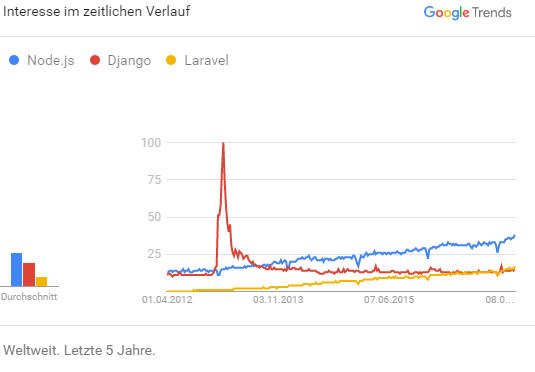
\includegraphics[width=3.8in]{images/framework_trends}
    \caption{Google Trends der evaluierten Frameworks\cite{frameworks_trends}}
\end{figure}

\newpage

%%%%%%%%%%%%%%%%%%%%%%%%%%%%%%%%%%%%%
%         Datenübermittlung         %
%%%%%%%%%%%%%%%%%%%%%%%%%%%%%%%%%%%%%
\subsection{Art der Daten\"ubermittlung}
Bei der Daten\"ubertragung sind mehrere Parameter zu beachten. Dazu geh\"oren haupt-s\"achlich das Format der Daten und das Intervall in denen diese \"ubertragen werden.
\subsubsection{Arduino zu Raspberry Pi und vice versa}
Um die Sensordaten dem Raspberry Pi mitzuteilen, eignet sich am besten ein Key-Value Format. Dabei gibt es verschiedene M\"oglichkeiten, wie z.B. \gls{JSON} und \gls{CSV}. \\
Das Intervall der Daten\"ubertragung kann frei, vom Benutzer gew\"ahlt werden.
\paragraph{\gls{JSON}} \mbox{}\\
\gls{JSON} (JavaScript Object Notation) hat den gro{\ss}en Vorteil, der leichten Server-seitigen Auswertung und Konvertierung in ein Javascript Objekt. Da die Daten aber \\ vorübergehend auf dem Raspberry Pi persistiert werden sollen, und Redis kein automatisches speichern von \gls{JSON} Objekten unterst\"utzt erzeugt diese Methode der \"Ubertragung mehr Aufwand als Nutzen.
\paragraph{\gls{CSV}} \mbox{}\\
\"Ahnlich wie bei \gls{JSON}, m\"ussten die Daten erst bearbeitet und gefiltert werden, um in die Datenbank gespeichert werden zu k\"onnen.
\paragraph{Eigenes Format} \mbox{}\\
Da die Daten in einer Redis Datenbank auf dem Key-Value Prinzip basieren, können die Daten auch entsprechend übertragen werden. Ein Key-Value-Paar wird in einer Zeile übertragen ("`ph 7.2\textbackslash n"')
\paragraph{Fazit} \mbox{}\\
Der Datenaustausch zwischen Arduino und Raspberry Pi wird in folgendem Format stattfinden:
\begin{lstlisting} [frame=single, caption=Datenaustauschformat zwischen Raspberry Pi und Arduino]
	tp 18.2
	ph 7.2
	ec 286.4
\end{lstlisting}

\newpage
\subsubsection{Raspberry Pi zu Server und vice versa}
Nachdem die Daten in Redis gespeichert wurden, werden diese zum Zentralserver gesendet. Node.js wird sowohl als Client als auch als Empfänger verwendet.

Die Daten sehen bei Auslesen der Datenbank wie folgt aus:
\begin{lstlisting} [frame=single, caption=Daten beim Auslesen der Datenbank]
	1) tp
	2) 23.4
	3) ec
	4) 285.7
\end{lstlisting}

Wie in Kapitel 4.6.1 festgestellt, offenbart sich die \"Ubertragung in \gls{JSON} nicht nur wegen der Einfachheit der Konvertierung zu einem Javascript Objekt als Vorteil, sondern auch aus drei anderen Gr\"unden:
\begin{itemize}
    \item \textbf{Einfache Speicherung in MongoDB:} Da MongoDB \gls{JSON} als Speicherformat verwendet, ist es deswegen f\"ur uns einfacher \gls{JSON}-Objekte in die Datenbank zu speichern.
    \item \textbf{\"Ubertragung der Daten durch Socket.io:} Daten werden standardm\"a{\ss}ig in Socket.io als \gls{JSON}-Objekt gesendet.
    \item \textbf{Oberfl\"ache der Webapp durch Angular:} Angular bietet Funktionen an, \gls{JSON}-Objekte in der Weboberfl\"ache anzeigen zu lassen. Falls sich das \gls{JSON}-Objekt ver\"andert, wird automatisch auch die Oberfl\"ache dementsprechend angepasst.
\end{itemize}

Deswegen werden die Daten wie folgt aussehen:
\begin{lstlisting} [frame=single, caption=Datenformat]
	{
	  tp: "23.4",
	  ec: "285.7"
	}
\end{lstlisting}
\newpage
\subsection{Komponenten- und Kostenaufstellung}
Die Gesamtkosten ergeben sich aus den Unterpunkten Technik, Zubehör und Webpräsenz:
\begin{table}[ht]
{\centering
\begin{tabular}{c|c}
Summe Technik    & 313,78 € \\
Summe Zubehör    & 186,78 € \\
Summe Webpräsenz & 50,00 €  \\ \hline
\textbf{Gesamtbetrag}     & \textbf{550,56 €}
\end{tabular}
\caption{Gesamtsumme der Kosten}}
\end{table}

\mbox{} \\
Die Kosten, um unsere Webpräsenz, sowie die Web-App, zu hosten, belaufen sich auf folgende Unterpunkte:
\mbox{} \\

\begin{table}[ht]
{\centering
\begin{tabular}{|c|c|}
\hline
\textbf{Artikel}       & \textbf{Einkaufspreis} \\ \hline
Server OVH-VPS         & 20,00 € per 6 Monate   \\ \hline
Domain (urbangreen.io) & 30,00 € pro Jahr       \\ \hline
\end{tabular}
\caption{Webpräsenz Kosten}}
\end{table} \mbox{} \\
In der unten stehenden Tabelle sind alle verbauten Komponenten, dessen Stückzahl und Einkaufspreis gelistet:\\

\begin{table}[ht]
\centering
\begin{tabular}{|c|c|c|}
\hline
\textbf{Artikel}                                                                                     & \textbf{Stückzahl} & \textbf{Gesamtpreis}   \\ \hline
\begin{tabular}[c]{@{}c@{}}Raspberry Pi Display\end{tabular}                                         & 1                  & 80,00 €                \\ \hline
\begin{tabular}[c]{@{}c@{}}Aquariumheizer, Eheim Thermocontrol\\ 200 Watt\end{tabular}               & 1                  & 22,99 €                \\ \hline
Luftpumpe, Eheim air pump 400                                                                        & 1                  & 27,99 €                \\ \hline
\begin{tabular}[c]{@{}c@{}}Außenpumpe, JBL Cristalprofi\\ E901\end{tabular}                          & 1                  & 89,00 €                \\ \hline
\gls{SBC}, Raspberry Pi 3B                                                                           & 1                  & 39,00 €                \\ \hline
Netzteil für Raspberry Pi 3B                                                                         & 1                  & 20,00 €                \\ \hline
RGB-LED Streifen                                                                                     & 1 (10 m)           & 25,00 €                \\ \hline
Jumperkabel                                                                                          & 1 (20 Stück)       & 5,00 €                 \\ \hline
Niedervoltbuchse                                                                                     & 1                  & 3,00 €                 \\ \hline
\gls{MOSFET}                                                                                         & 3                  & 1,80 €                 \\ \hline
\textbf{Gesamtsumme}                                                                                          & \textbf{-}                  & \textbf{313,78 €}               \\ \hline
\end{tabular}
\caption{Kostenaufstellung technische Einkäufe für den Prototypen}
\end{table}

\newpage
Um das Aquarium zu betreiben und Wartbarkeit beizubehalten, mussten diverse Artikel angeschafft werden. Diese Artikel umfassen diverse Wasseraufbereiter und Wasserpflegemittel, Aquariumkies und -sand aber ein Transportroller welcher ermöglicht das Aquarium, wenn benötigt (bei Wartarbeiten oder zum Beispiel Übersiedlung), erleichtert zu transportieren.\\
All diese gekauften Artikel werden in der folgenden Tabelle aufgelistet:
\begin{table}[ht]
\centering
\begin{tabular}{|c|c|c|}
\hline
\textbf{Artikel}                                                                     & \textbf{Stückzahl} & \textbf{Gesamtpreis}   \\ \hline
\begin{tabular}[c]{@{}c@{}}Aquarien Pflanzensand, \\ JBL Aquabasis plus\end{tabular} & 1 (5 l)            & 12,99 €                \\ \hline
Aquariumsand                                                                         & 2 * 4,5 l          & 8,98 €                 \\ \hline
Aquariumkies                                                                         & 2                  & 15,98 €                \\ \hline
\begin{tabular}[c]{@{}c@{}}Kunststoff Baumstamm\\ Fischversteck\end{tabular}         & 1                  & 17,99 €                \\ \hline
Keramik Fischversteck                                                                & 1                  & 16,99 €                \\ \hline
Deko Holzwurzelstamm                                                                 & 1                  & 12,99 €                \\ \hline
Deko Calari Stein                                                                    & 1                  & 5,95 €                 \\ \hline
Aquariumpflanzen                                                                     & 4                  & 11,16 €                \\ \hline
Aquariumschwamm JBL Spongi                                                           & 1                  & 1,95 €                 \\ \hline
AquaForte Eco-Check Teststreifen                                                     & 1 (50 Stück)       & 10,90 €                \\ \hline
Filtergel                                                                            & 1 (0,5 l)          & 12,50 €                \\ \hline
Aquariumreiniger, Sludge-Away                                                        & 1 (1 l)            & 16,50 €                \\ \hline
Eisendünger 6\%                                                                      & 1 (70 g)           & 5,00 €                 \\ \hline
\begin{tabular}[c]{@{}c@{}}Transportroller, \\Bauhaus Eigenmarke bis zu \\400 kg Traglast\end{tabular}                           & 1                  & 36,90 €                \\ \hline
\textbf{Gesamtsumme}                                                                          & \textbf{-}                  & \textbf{186,78 €}               \\ \hline
\end{tabular}
\caption{Aquarium Zubehör}
\end{table}

Die Entwicklung des System benötigt keine zusätzlichen Kosten, welche beispielsweise für Lizenzen benötigt werden.

\newpage
\subsection{Fazit des kompletten Systems}

Der Aufbau des kompletten System wurde in der folgenden Grafik veranschaulicht und basiert auf die Evaluierung.

\begin{figure}[ht]
    \centering
    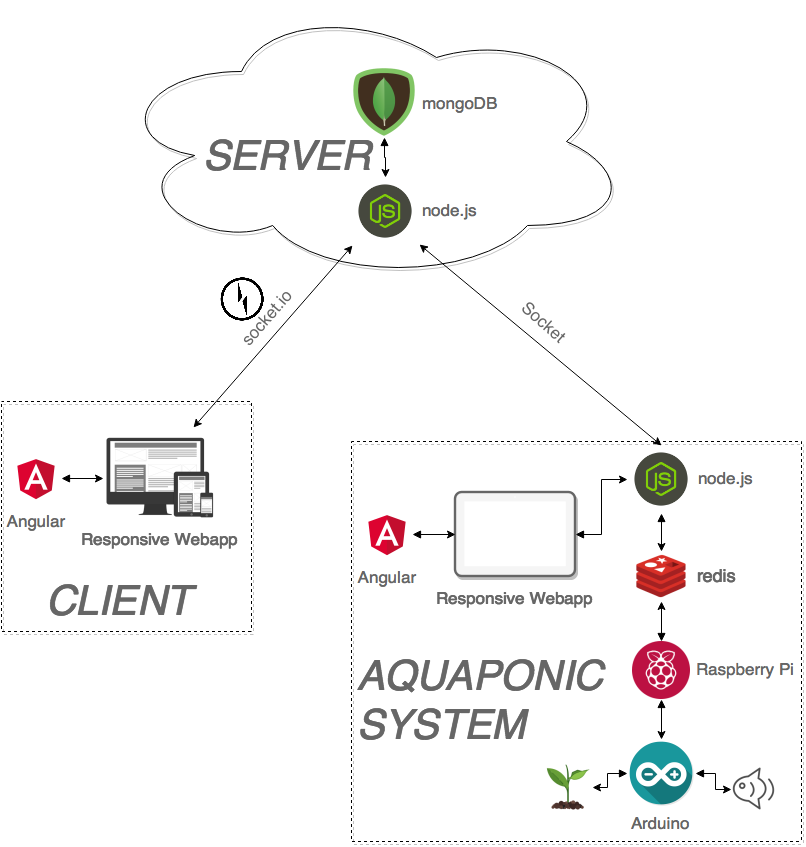
\includegraphics[height=5.5in]{images/complete_system}
    \caption{Aufbau komplettes System}
\end{figure}



\afterpage{\blankpage}

\newpage %----------------------------------------------------------------------------------------------
\section{Projekt Umsetzung - Designunterlagen}
%\input{}

\subsection{Use-Case Diagramm}
%\input{}

\subsection{Datenakquisition}
%\input{}

\subsubsection{Technologie}
%\input{}

\subsubsection{Ablauf}
%\input{}

\subsection{Datenverarbeitung}
%\input{}

\subsubsection{Technologie}
%\input{}

\subsubsection{Umsetzung des Ablaufs}
%\input{}


\newpage %----------------------------------------------------------------------------------------------
\section{Zugriff auf das Aquaponik Systems}
%\input{}

\subsection{Userinterface - Frontend}
\subsubsection{User Experience}
\subsubsection{Browserkompatibilität}
\subsubsection{Technologien}
\subsubsection{Funktionen}
\subsubsection{Optimierungen}
\subsection{Zentralserver}
\subsubsection{Authentifikation}
\subsubsection{Kommunikation}
%\input{}

\newpage %----------------------------------------------------------------------------------------------
\section{Ausfallsicherheit und Konsistenzsicherung der Daten}
%\input{}

\subsection{Zwischenspeicherung beim Aquaponik System}
%\input{}

\subsubsection{Ausfall der Internetverbindung}
%\input{}

\subsubsection{Ausfall der Stromversorgung}
%\input{}

\newpage %----------------------------------------------------------------------------------------------
\section{Prototyp testing}
\subsection{Hardware}
\subsection{Prototyp}
\subsection{Aussichten}
%\input{}

\newpage %----------------------------------------------------------------------------------------------
\section{Ausblick}
%\input{}

\newpage %----------------------------------------------------------------------------------------------
\cfoot{}
\pagenumbering{roman}
\section{Appendix}
\label{sec:appenix}

\subsection{Glossaries}
\label{subsec:glossaries}
\begingroup
\renewcommand{\section}[2]{}
\printglossary[style=tree]
\endgroup
\newpage

{\small\color{white}.}
\vspace{-2cm}
\subsection{Figures}
\label{subsec:figures}
\begingroup
\renewcommand{\section}[2]{}
\listoffigures
\endgroup

\subsection{Listings}
\label{subsec:listings}
\begingroup
\renewcommand{\section}[2]{}
\lstlistoflistings
\endgroup

\subsection{Sources}
\label{subsec:sources}
\begingroup
\renewcommand{\section}[2]{}
\bibliographystyle{alpha}
\bibliography{sources}
\endgroup


\end{document}
